\documentclass[a4paper, 12pt, twoside, openright, fleqn,usenames, dvipsnames, table, tikz]{book}
%language settings
\usepackage[italian]{babel}
\usepackage[T1]{fontenc}

\usepackage[utf8]{inputenc}
% \usepackage{textgreek}
\usepackage{fancyhdr} % headers and footers

% figures and positioning
\usepackage{caption}
\usepackage{float}
\usepackage{graphicx}
\usepackage{graphics}
\usepackage{wrapfig}
\usepackage{listing}
\usepackage{pdfpages}
% math package
\usepackage{mathtools}
\usepackage{amsthm, environ}%
\usepackage{amsmath, amssymb, dsfont, bm,blkarray}%
\usepackage{cases}

% tikz figures
\usepackage{tikz,pgfplots}
\usetikzlibrary{shapes, arrows,automata}
\usepackage{xcolor}

% image path
\usepackage{epstopdf}
\graphicspath{ {./img/} }

% add support for url and cross-references in PDF output
\usepackage{url}
\renewcommand{\UrlFont}{\color{black}\small\ttfamily}
\usepackage[colorlinks=true, linkcolor=black, citecolor=black, urlcolor=black]{hyperref}

% support for glossary and acronyms
\usepackage[acronym]{glossaries}
\newacronym[plural=MCs,firstplural=Markov Chains (MCs)]{mc}{MC}{Markov Chain}
\newacronym[plural=AF,firstplural=Array Factor (AF)]{af}{AF}{Array Factor}
\newacronym[plural=SLL,firstplural=Side Lobe Levels (SLL)]{sll}{SLL}{Side Lobe Level}
\newacronym{eirp}{EIRP}{Effective Isotropic Radiated Power}
\newacronym{pec}{PEC}{Perfect Electric Conductor}

% Costumization of theorem style
\newtheoremstyle{theoremdd}% name of the style to be used
  {\topsep}% measure of space to leave above the theorem. E.g.: 3pt
  {\topsep}% measure of space to leave below the theorem. E.g.: 3pt
  {\itshape}% name of font to use in the body of the theorem
  {0pt}% measure of space to indent
  {\bfseries}% name of head font %\color{Mahogany}
  { -- }% punctuation between head and body
  { }% space after theorem head; " " = normal interword space
  {\thmname{#1}\thmnumber{ #2}\thmnote{ (#3)}}

\theoremstyle{theoremdd}
% support for counting
\newtheorem{theorem}{Teorema}[section]
\newtheorem{corollary}{Corollario}[theorem]
\newtheorem{lemma}[theorem]{Lemma}
\newtheorem{definition}{Definizione}
\newtheorem{remark}{Nota}


% added support for proof parts
\theoremstyle{remark}
\newtheorem{proofpart}{Part}
\renewcommand\theproofpart{\Roman{proofpart}}
\makeatletter%
\@addtoreset{proofpart}{theorem}%
\makeatother

% specific modification to basic book template of our book document
\renewcommand{\chaptername}{Section}
\addto\captionsenglish{\renewcommand{\chaptername}{Section}}
\renewcommand\qedsymbol{\includegraphics[width=1.5cm]{occhiali}}
%\renewcommand\qedsymbol{$\square$\itshape QED}

% alias for differentials
\newcommand*\de{\mathop{}\!\mathrm{d}}

% useful aliases for common employed declarations
\def \beq {\begin{equation}}
\def\eeq{\end{equation}}
\def\bal{\begin{align}}
\def\eal{\end{align}}
\def\prob{\ensuremath\mathbb{P}}%
\def\exp{\ensuremath\mathbb{E}}
\newcommand{\Hb}{\mathbb{H}}
\newcommand{\Sb}{\mathbb{\Sigma}}
\newcommand{\U}{\mathbb{U}}
\newcommand{\F}{\mathbb{F}}
\newcommand{\V}{\mathbb{V}}
\newcommand{\A}{\mathbb{A}}
\newcommand{\B}{\mathbb{B}}
\newcommand{\C}{\mathbb{C}}
\newcommand{\E}{\mathbb{E}}
\newcommand{\I}{\mathbb{I}}
\newcommand{\Y}{\mathbb{Y}}
\newcommand{\N}{\mathbb{N}}
\newcommand{\W}{\mathbb{W}}
\newcommand{\Z}{\mathbb{Z}}
\newcommand{\R}{\mathbb{R}}
\newcommand{\X}{\mathbb{X}}
\newcommand{\Pb}{\mathbb{P}}
\newcommand{\Q}{\mathbb{Q}}
\newcommand{\D}{\mathbb{D}}
\newcommand{\Rm}{\mathbb{R^{-1}}}
\newcommand{\J}{\mathbb{J}}
\newcommand*{\Chi}{\raisebox{2pt}{\mbox{\Large $\chi$}}}% big chi
\newcommand{\Fig}[1]{Fig.~\ref{#1}}
\newcommand{\eq}[1]{(\ref{#1})}
\newcommand{\Tab}[1]{Tab.~\ref{#1}}
\newcommand{\Sec}[1]{Sec.~\ref{#1}}
\newcommand{\indep}{\mathrel{\perp\mspace{-10mu}\perp}}
\newcommand{\RN}[1]{ \textup{\uppercase\expandafter{\romannumeral#1}}} %This is for inserting Roman Numbers (useful for \stackrel in equations so that you don't confuse indicating numbers from equation numbers
\newcommand{\e}{\ensuremath{\vec{e}}}
\newcommand{\ert}{\ensuremath{\vec{e}(\vec{r},t)}}
\renewcommand{\b}{\ensuremath{\vec{b}}}
\newcommand{\brt}{\vec{b}(\vec{r},t)}
\newcommand{\h}{\ensuremath{\vec{h}}}
\newcommand{\hrt}{\ensuremath{\vec{h}(\vec{r},t)}}
\renewcommand{\d}{\ensuremath{\vec{d}}}
\newcommand{\drt}{\ensuremath{\vec{d}(\vec{r},t)}}
\newcommand{\jt}{\ensuremath{\vec{j}_T}}
\renewcommand{\r}{\ensuremath{\vec{r}}}
\newcommand{\s}{\ensuremath{\vec{s}}}
\renewcommand{\a}{\ensuremath{\vec{a}}}
\renewcommand{\k}{\ensuremath{\vec{k}}}
\newcommand{\rot}{\ensuremath{\nabla\times}}
\newcommand{\diverg}{\ensuremath{\nabla\cdot}}
\renewcommand{\E}{\ensuremath{\vec{E}}}
\renewcommand{\H}{\ensuremath{\vec{H}}}
\renewcommand{\J}{\ensuremath{\vec{J}}}
\newcommand{\M}{\ensuremath{\vec{M}}}
\renewcommand{\A}{\ensuremath{\vec{A}}}
\renewcommand{\S}{\ensuremath{\vec{S}}}
\renewcommand{\P}{\ensuremath{\vec{P}}}
% riduzioni antenne
\newcommand{\hhat}[1]{\,\hat{#1}}
\newcommand{\hz}{\ensuremath{\hhat{z}}}
\newcommand{\hth}{\ensuremath{\hhat{\theta}}}
\newcommand{\hphi}{\ensuremath{\hhat{\phi}}}
\newcommand{\hr}{\ensuremath{\hhat{r}}}
\newcommand{\ejbr}{\ensuremath{e^{-\jmath \beta r}}}
\newcommand{\ejbrp}{\ensuremath{e^{\jmath \beta r}}}
\newcommand{\oqme}{\ensuremath{\omega^2 \mu \epsilon}}
\newcommand{\pvec}[1]{\ensuremath{\vec{#1}\mkern2mu\vphantom{#1}^\prime}}
\newcommand{\rp}{\pvec{r}}
\DeclareMathOperator{\ctg}{ctg}

% nice tables settings
\usepackage{booktabs}
\newcolumntype{C}[1]{>{\centering\let\newline\\\arraybackslash\hspace{0pt}}m{#1}}

% multiple subfigure in figures
\usepackage{subcaption}

% Derivatives shortcut
\newcommand{\deriv}[3][]{% \deriv[<order>]{<func>}{<var>}
  \ensuremath{\frac{\partial^{#1} {#2}}{\partial {#3}^{#1}}}}
%---------------------------------
\NewEnviron{esp}{%
\begin{equation}\begin{split}
  \BODY
\end{split}\end{equation}
}

\NewEnviron{esp*}{%
\begin{equation*}\begin{split}
  \BODY
\end{split}\end{equation*}
}

% no newline inside $...$ inline formula
\binoppenalty=\maxdimen
\relpenalty=\maxdimen

\begin{document}

% custom autoref for equations and figures
\def\equationautorefname~#1\null{(#1)\null}
\def\figureautorefname~#1\null{figura #1\null}
\def\tableautorefname~#1\null{tabella #1\null}

\begin{titlepage}
	\begin{center}
		\hspace{0.5cm}
		\Large{Antenne e propagazione wireless} \\
		\vspace{1cm}
		%\includegraphics[width=9cm]{Zorzilla}\\
		\vspace{0.5cm}
		\emph{written with love by} \\
		\vspace{0.5cm}
		{\Large Andrea Pittaro, Enrico Lovisotto, Umberto Martinelli}
	\end{center}

	\vfill

	\begin{center}
		\line(1, 0){360}

		\textsc{Anno Accademico 2016/2017}
	\end{center}
\end{titlepage}

\tableofcontents
\clearpage

\chapter{Introduction}
\section{Topics of the course}
\begin{itemize}
  \item Review of probability theory
  \item Markov chains
  \item Poisson processes
  \item Example of applications protocols
  \item Random access protocols
\end{itemize}
\section{Review of probability theory}
Let $X_n, X_t$ be two different instances of a random variable (r.v.). We will use
\textit{t} as a subscript if the r.v. is continuous ($t \in \mathbb{R}$), \textit{n} if the r.v. is discrete ($ n \in \mathbb{Z}$)

Let \textit{A},\textit{B} be two events, then:
\begin{itemize}
  \item if $A \cap B = \emptyset$, then A and B are disjoint
  \item $P[A \cup B] = P[A]+P[B] - P[A \cap B]$
  \item $0\le P[A] \le 1$
  \item $P[A \cup B] \le P[A]+P[B]$
  \item $ P[\Omega]=1 $ and $P[\emptyset]=0$ with $\Omega$ the Universe set
\end{itemize}
\subsection{Total probability law}
Given $A_i \cap A_j = \emptyset \;\; \forall i \neq j $, then $\bigcup\limits_{i=1}^{+\infty} A_i \, = \Omega$.
Moreover $P[B]=\sum\limits_{i=1}^{+\ifty} P[B \cap A_i]$.

If $P[A \cap B] = P[A]\cdot P[B] \implies A,B$ \textit{are} \textbf{independent}.

\subsection{Distribution function (PMD)}\label{sec:pmd}
$F(x) = P[X \le x]$ is called the distribution function and has the following properties:
\begin{enumerate}
  \item $\lim\limits_{x \to -\infty} F(x) = 0$ \quad and \quad $\lim\limits_{x \to +\infty} F(x) = 1$
  \item F is monothonic non-decreasing $\implies$ if $x_1 > x_2 \implies F(x_1)\ge F(x_2)$
  \item F(x) is continuous from the right
\end{enumerate}
We define $f(x)=F'(x)$ the probability density function \textit{PDF}.

\subsection{Moment}
We define  the moment as:
$E[X^m]=
\begin{cases}
    \sum\limits_{i} {x{_i}^{m} \cdot P[X=x_i]} & \text{if X is discrete } \\
    \int_{-\infty}^{+\infty} {x^{m} \cdot f(x) dx }  & \text{if X is continuous}
\end{cases}$
In particular if m=1, we obtain the mean, if m=2 we get the power (and in particular if $E[X]=0$ we obtain the variance).\\
Defining $\mu = E[X]$, we say that $E[(X-\mu)^m]$ is the center moment.\\
We will denote $E[g(x)]=\int_{-\infty}^{+\infty} g(x)\, d F_X(x)$

\subsection{Joint probability}
We define the joint probability of two variables as
\begin{equation*}
  $$F_{XY}(x,y)=P[X\le x , Y \le y] \stackrel{\text{cont. case}}{=} \int_{-\infty}^{+\infty}\int_{-\infty}^{+\infty} f_{XY}(\eta,\xi) d\eta d\xi$$
\end{equation*}

From what we obtain in \ref{sec:pmd}, we can write \\
\begin{equation*}
  $$F_X(x)=F_{XY}(x,+\infty)=\lim\limits_{y \to +\infty} F_{XY}(x,y)$$
  $$F_Y(y)=F_{XY}(+\infty,y)=\lim\limits_{x \to +\infty} F_{XY}(x,y)$$
\end{equation*}
If X and Y are independent ($X \indep Y$), we have
\begin{itemize}
  \item $F_{XY}(x,y)=F_X(x)\cdot F_Y(y) \; \forall x,y$
  \item $cov(X,Y) = E[(X - \mu_X)\cdot (Y - \mu_Y)] = E[X \cdot Y]-\mu_X \cdot \mu_Y$
\end{itemize}
If X and Y are uncorrelated ($X \bot Y$) $\implies cov(X,Y)=0$.

\subsection{Conditional probability}

\chapter{Polarizzazione del campo \textsc{EM}}
Andremo ora ad analizzare come si comporta il campo elettromagnetico nello spazio, in particolare la sua evoluzione e i casi degeneri.

Iniziamo con un'analisi nel dominio del tempo del campo, prestando attenzione alla differenza con il corso di Fisica 2: mentre nell'altro corso si è osservata la polarizzazione del mezzo, ora analizzeremo la polarizzazione dell'onda elettromagnetica.
\begin{esp}
  \ert &= \sum\limits_{n=1}^3 \hat{x}_n^{\prime\prime} \cdot \E_n(\r)\cdot cos\left[\omega t + \phi_{E_n}(\r)\right] \\
  &= \sum\limits_{n=1}^3 \hat{x}_n^{\prime\prime} \cdot \E_n(\r)\cdot cos(\omega t)\cdot cos\left[ \phi_{E_n}(\r)\right] - sin(\omega t)\cdot sin\left[ \phi_{E_n}(\r)\right]\\
  &=cos(\omega t) \cdot \sum\limits_{n=1}^3 \hat{x}_n^{\prime\prime} \cdot \E_n(\r)\cdot cos \left[ \phi_{E_n}(\r) \right] \\
  &+sin(\omega t) \cdot \sum\limits_{n=1}^3 \hat{x}_n^{\prime\prime} \cdot \E_n(\r)\cdot sin \left[ \phi_{E_n}(\r) \right] \\
\end{esp}

Raggruppando i termini, si ha in conclusione che
\begin{equation} \label{eq:ert}
	\ert = \E^R(\r)\cdot cos(\omega t) - \E^I(\r)\cdot sin(\omega t)
\end{equation}

\newpage
con il vettore di Steinmetz del campo elettrico scomposto in parte reale e immaginaria
\begin{equation*} \begin{dcases}
	\E^R(\r) &= \sum\limits_{n=1}^3 \hat{x}_n^{\prime\prime} \cdot \E_n(\r)\cdot cos \left[ \phi_{E_n}(\r) \right] \\
	\E^I(\r) &= \sum\limits_{n=1}^3 \hat{x}_n^{\prime\prime} \cdot \E_n(\r)\cdot sin \left[ \phi_{E_n}(\r) \right]
\end{dcases} \end{equation*}

Possiamo osservare il vettore di Steinmetz si può ottenere direttamente dalla formula del campo
\begin{equation*} \begin{dcases}
	\e(\r, t=0) = \E^R(\r) \\
	\e \left( \r, t = \frac{pi}{2\omega} \right) = -\E^I(\r)
\end{dcases} \end{equation*}

\paragraph{Proprietà di polarizzazione del campo}
A partire dall'equazione \ref{eq:ert} possiamo osservare alcune simmetrie del campo $\E$:
\begin{enumerate}
  \item il campo elettromagnetico giace sempre su un piano di polarizzazione, qualunque $t$ si scelga
  \item il campo elettromagnetico traccia una curva chiusa
  \item la curva chiusa è, in generale, un ellisse
\end{enumerate}

Queste affermazioni possono essere provate come segue
\begin{esp}
  \E^R &= E^R_{x^{\prime}} \cdot \hat{x}^{\prime}+E^R_{y^{\prime}} \cdot \hat{y}\prime \\
  \E^I &= E^I_{x^{\prime}} \cdot \hat{x}^{\prime}+E^I_{y^{\prime}} \cdot \hat{y}\prime \\
  \e &= (E^R_{x^{\prime}}\cdot \hat{x}^{\prime}+ E^R_{y^{\prime}})\cdot cos(\omega t) - (E^I_{x^{\prime}}\cdot \hat{x}^{\prime}+ E^I_{y^{\prime}})\cdot sin(\omega t)\\
  &= \left[E^R_{x^{\prime}} \cdot cos(\omega t)-E^I_{x^{\prime}}\cdot sin(\omega t)\right]\cdot \hat{x}^{\prime} + \left[E^R_{y^{\prime}} \cdot cos(\omega t) -E^I_{y^{\prime}}\cdot sin(\omega t)\right]\cdot \hat{y}\prime \\
\end{esp}
  o in forma matriciale
\begin{esp}
  \begin{pmatrix}
    e_{x^{\prime}} \\ e_{y^{\prime}}
  \end{pmatrix}
  &=
  \underbrace{\begin{pmatrix}
    E_{x^{\prime}}^R & -E_{x^{\prime}}^I\\
    E_{y^{\prime}}^R & -E_{y^{\prime}}^I
  \end{pmatrix}}_{\text{Deformazione lineare}}
  \cdot
  \underbrace{\begin{pmatrix}
    cos(\omega t) \\ sin(\omega t)
  \end{pmatrix}}_{\text{circonferenza}}
\end{esp}

Passando quindi alle coordinate cartesiane principali, si ottiene
\begin{esp}
\begin{pmatrix} e_{x} \\ e_{y} \end{pmatrix}
&= \begin{pmatrix}
  a \cdot cos(\omega t + \Phi) \\
  \pm b \cdot sin(\omega t + \Phi)
\end{pmatrix}
\end{esp}
dove $a,b \in \R^+$ indicano il valore dei semiassi dell'ellisse, mentre il $\pm$ indica il verso \emph{destrorso} o \emph{sinistrorso} della polarizzazione ellittica del campo elettrico. Ci sono ora due casi degeneri principali:
\begin{enumerate}
  \item $a = b$ l'ellisse degenera in una circonferenza, per cui la polarizzazione sarà circolare destrorsa o sinistrorsa
  \item $\begin{cases}a=0 \\ b \neq 0 \end{cases} \vee  \begin{cases}a\neq 0 \\ b = 0 \end{cases}$ l'ellisse degenera in un segmento e la polarizzazione sarà rettilinea verticale o orizzontale.
\end{enumerate}

Queste proprietà si posso ricavare anche con i vettori di Steinmetz
\begin{esp}
  \e(t) &= \Re[\E\cdot e^{\jmath \omega t}] \quad \E \in \C^3 \\
  &=\Re\left[\left(\E^R + \jmath \E^I\right)\cdot\left(\cos(\omega t) + \jmath \sin(\omega t)\right)\right] \\
	&= \E^R \cdot cos(\omega t) - \E^I\cdot sin(\omega t) \\
  &= a \cdot cos(\omega t + \Phi)\cdot \hat{x} \pm b \cdot sin(\omega t + \Phi)\cdot \hat{y}
\end{esp}

Ruotando il sistema di riferimento di un angolo $\delta$ la proprità resta valida: è sufficiente applicare la corrispodente trasformazione ai campi considerati.
\begin{equation}
  \begin{pmatrix} E_{x^{\prime}} \\ E_{y^{\prime}} \end{pmatrix} =
  \begin{pmatrix}
     cos(\delta) & sin(\delta) \\ -sin(\delta) & cos(\delta)
  \end{pmatrix} \cdot
    \begin{pmatrix} E_{x} \\ E_{y} \end{pmatrix}
\end{equation}

\section{Rapporto di polarizzazione rettilinea}
Definiamo il rapporto di polarizzazione $p$ nel sistema di assi principali come
\begin{equation}
  p = \jmath \frac{E_y}{E_x} \in \C
\end{equation}
mentre in un sistema di assi generico, si ottiene, in modo analogo alle linee di trasmissione,
\begin{equation}
  p\prime = \jmath \frac{E_y}{E_x} = \frac{p - \jmath tg(\delta)}{1-\jmath p \cdot tg(\delta)}
\end{equation}
Risulta interessante notare come, per qualsiasi angolo $\delta$ il segno di $p\prime$ non cambi. $p\prime \in \C$ discrimina infatti, indipendentemente dal sistema di referimento, i diversi tipi di polarizzazione
\begin{equation}\begin{cases}
  \Re[p\prime] >0 & \text{ellittica destrorsa} \\
  \Re[p\prime] <0 & \text{ellittica sinistrorsa} \\
  \Re[p\prime] =0 & \text{rettilinea ``orizzontale''} \\
  \Re[p\prime] =\infty & \text{rettilinea ``verticale''} \\
  p = p\prime = 1 & \text{circolare destrorsa} \\
  p = p\prime = 1 & \text{circolare sinistrors}
\end{cases}\end{equation}

% \textbf{\textsc{Nota Bene}} la polarizzazione circolare prevede che $p=p\prime$ sia \textbf{puramente reale} e pari a $\pm1$

Cerchiamo ora di valutare $\Re [p\prime]$
\begin{esp*}
  p\prime
	&= \jmath \frac{E_{y^{\prime}}}{E_{x^{\prime}}} \\
	& = e^{\jmath \frac{\pi}{2}} \cdot \left \| \frac{E_{y^{\prime}}}{E_{x^{\prime}}} \right \|
  \cdot e^{j(\Phi_{y^{\prime}}-\Phi_{x^{\prime}})} \\
  &= \left \| \frac{E_{y^{\prime}}}{E_{x^{\prime}}} \right \| \cdot e^{j(\frac{\pi}{2}+\Phi_{y^{\prime}}-\Phi_{x^{\prime}})}
\end{esp*}

e dunque,
\begin{esp*}
	\Re[p\prime]
	&= \left \| \frac{E_{y^{\prime}}}{E_{x^{\prime}}} \right \| \cdot \underbrace{\cos \left( \frac{\pi}{2} +\Phi_{y^{\prime}}-\Phi_{x^{\prime}} \right)}_{\text{verso di polarizzazione}}
\end{esp*}

\chapter{Onde piane}
Le onde piane sono particolari soluzioni delle equazioni di Maxwell che hanno proprietà e simmetrie notevoli che ne semplificano notevolmente lo studio rispetto al caso generale.

\section{Equazioni di Helmotz}
	Le equazioni di Maxwell possono essere riscritte come le cosiddette equazioni di Helmotz, nel caso in cui il mezzo sia il vuoto.

	\begin{equation*}
		\begin{cases}
			\rot\E = - \jmath \, \omega \, \mu \, \H \\
			\rot\H = \jmath \, \omega \, \epsilon_c \, \E \\
		\end{cases}
	\end{equation*}

	Applicando, per esempio alla prima, l'operazione di rotore ad ambo i membri, e sostituendo la seconda si ottiene
	\begin{equation*}
		\begin{split}
			\rot\rot\E &= - \jmath \, \omega \, \mu \, \rot \rot\H \\
			- \nabla^2\E &= - \jmath \, \omega \, \mu \, (\jmath \, \omega \, \epsilon_c \, \E)\\
		\end{split}
	\end{equation*}

	\begin{equation} \label{eq:helmotz}
		\begin{cases}
			\nabla^2 \E + \omega^2 \, \mu \, \epsilon_c \, \E = 0 \\
			\nabla^2 \H + \omega^2 \, \mu \, \epsilon_c \, \H = 0
		\end{cases}
	\end{equation}

	Esse sono affini alle ben note equazioni delle onde: la loro soluzione sarà perciò nella forma

	\begin{equation} \label{eq:helmotz_sol}
		\begin{cases}
			E_x(\r) = E_{ox} ~ e^{-\s \cdot \r} \\
			E_y(\r) = E_{oy} ~ e^{-\s \cdot \r} \\
			E_z(\r) = E_{oz} ~ e^{-\s \cdot \r}
		\end{cases}
	\end{equation}
	dove $\r$ è il vettore reale che definisce la posizione del punto considerato, mentre $\s = (s_x, s_y, s_z)$ è detto vettore \emph{di spostamento} e definisce come il campo vari nello spazio in modulo e fase.

	Sostituendo questa generica soluzione in \ref{eq:helmotz}, si ottiene la condizione che il parametro $\s$ deve soddisfare per essere un'effettiva soluzione.

	\begin{equation} \label{eq:condizione_s}
		\begin{split}
			& \nabla^2 E_x+ \omega^2 \, \mu \, \epsilon_c \, E_x = 0 \\
			& E_{ox} ~ ({s_x}^2 e^{-\s \cdot \r} +
				{s_y}^2 e^{-\s \cdot \r} +
				{s_z}^2 e^{-\s \cdot \r}) +
				\omega^2 \, \mu \, \epsilon_c \, E_{ox} ~ e^{-\s \cdot \r} = 0 \\
			& \s \cdot \s = {s_x}^2 + {s_y}^2 + {s_z}^2 = - \omega^2 \, \mu \, \epsilon_c
		\end{split}
	\end{equation}
	dove nell'ultimo passaggio la somma dei quadrati delle componenti di $\s$ è indicata, con un abuso di notazione, come il prodotto scalare ``reale'' nonstante $\s$ sia un vettore complesso.

	Una volta individuate le condizioni per la validità della soluzione \ref{eq:helmotz_sol}, si può stabilire il legame tra campo elettrico e magnetico.

	\begin{equation*}
		\begin{split}
			\H & = \frac {\rot\E}{- \jmath \omega \mu} =
				\frac {\rot(\vec{E_o} ~ e^{-\s \cdot \r})}{- \jmath \omega \mu} \stackrel{(1)}{=} \\
			& = \frac {(\rot\vec{E_o}) ~ e^{-\s \cdot \r} - \vec{E_o} \times \nabla e^{-\s \cdot \r})} {- \jmath \omega \mu} \stackrel{(2)}{=} \\
			& = \frac { \vec{E_o} \times ( \s ~ e^{-\s \cdot \r})} {- \jmath \omega \mu} = \frac { \s \times \vec{E_o}} {\jmath \omega \mu} ~ e^{-\s \cdot \r} = \frac { \s \times \vec{E}} {\jmath \omega \mu} \\
		\end{split}
	\end{equation*}
	dove (1) è dato dalla derivata del prodotto, mentre (2) è dovuto al fatto che, essendo $\vec{E_o}$ costante, il suo gradiente è nullo.

\section{Piani di simmetria}
	La soluzione di onda piana presenta particolari comportamenti lungo e trasversalmente le direzioni date dalla parte reale e immaginaria del vettore $\s$.

	\begin{equation*}
		\s = \a + \jmath \k
	\end{equation*}

	\begin{itemize}
		\item[|$\Delta\r \perp \a$ )] Lungo questa direzione, l'ampiezza dei campi $\E$ e $\H$ non cambia.

		\begin{equation*}
			\begin{split}
				|\E(\r + \Delta\r)| &= |\vec{E_o}| ~ e^{-\a \cdot (\r + \Delta\r)} = \\
				& = |\vec{E_o}| ~ e^{-\a \cdot \r} ~ e^{-\a \cdot \Delta\r} \stackrel{(*)}{=} \\
				& = |\vec{E_o}| ~ e^{-\a \cdot \r} = |\E(\r)|
			\end{split}
		\end{equation*}
		dove (*) è dato dal fatto che $\a \cdot \Delta\r = 0$ per costruzione.

		\item[|$\Delta\r \perp \k$ )] Lungo questa direzione, la fase dei campi $\E$ e $\H$ non cambia.

		\begin{equation*}
				\measuredangle \E(\r + \Delta\r) = -\k \cdot (\r + \Delta\r) \stackrel{(*)}{=} - \k \cdot \r = \measuredangle \E(\r)
		\end{equation*}
		dove (*) è dato dal fatto che $\k \cdot \Delta\r = 0$ per costruzione.

		\item[|$\Delta\r \parallel \a$ )] Lungo questa direzione, l'ampiezza dei campi cala in modo esponenziale in $|\a|$ e in $\Delta r$.

		\begin{equation*}
			\begin{split}
				|\E(\r + \Delta\r)| &= |\vec{E_o}| ~ e^{-\a \cdot (\r + \Delta\r)} = \\
				& = |\vec{E_o}| ~ e^{-\a \cdot \r} ~ e^{-\a \cdot \Delta\r} \stackrel{(*)}{=} \\
				& = \left( |\vec{E_o}| ~ e^{-|\a| \Delta\r} \right) e^{-\a \cdot \r} = |\E(\r)| ~ e^{-|\a| \Delta\r}
			\end{split}
		\end{equation*}
		dove (*) è dovuto al parallelismo tra $\a$ e $\Delta\r$.

		\item[|$\Delta\r \parallel \k$ )] Lungo questa direzione, la fase dei campi $\E$ e $\H$ oscilla periodicamente.

		\begin{equation*}
				\measuredangle \E(\r + \Delta\r) = -\k \cdot (\r + \Delta\r) \stackrel{(*)}{=} - \k \cdot \r - |\k| \Delta r = \measuredangle \E(\r) - |\k| \Delta r
		\end{equation*}
		dove (*) è dovuto al parallelismo tra $\k$ e $\Delta\r$.

		Come si può osservare da questa periodicità della fase, i piano cosiddetti equifase sono separati da una distanza $\lambda$ funzione di $|\k| \stackrel{.}{=} \beta$.

		\begin{equation} \label{eq:lunghezza_donda}
			\lambda = \frac{2 \pi}{|\k|} = \frac{2 \pi}{\beta} \text{ è definita come \emph{lunghezza d'onda}}
		\end{equation}
	\end{itemize}

\section{Onda piana nel vuoto}
	Studieremo qui la propagazione dell'onda piana in un mezzo che, come il vuoto, è un perfetto isolante, ovvero $\sigma = 0$.

	Scomponendo l'equazione \ref{eq:condizione_s}, si può ottenere il seguente sistema

	\begin{equation} \label{eq:s_components}
		\begin{dcases}
			& |\a|^2 - |\k|^2 = - \omega^2 \, \mu \, \epsilon \\
			& 2 \a \cdot \k = \omega^2 \, \mu \, \sigma = 0
		\end{dcases}
	\end{equation}

	La seconda equazione è risolta per ciascuno dei seguenti casi

	\begin{equation}\begin{cases}
		|\a| = 0 \\
		|\k| = 0 \\
		\a \perp \k
	\end{cases}\end{equation}

	Il caso $|\k| = 0$ è da escludere a priori, perché la prima equazione del sistema \ref{eq:s_components} diventa impossibile.

	\subsection{Onda piana uniforme}
		Concentriamoci sul caso $|\a| = 0$: esso porta alla soluzione cosiddetta di onda piana uniforme, che si propaga nel vuoto senza perdite di potenza.

		\begin{equation*}
				\a = 0 \implies |\k| = \sqrt{\omega^2 \mu \epsilon} = \omega \sqrt{\mu \epsilon} = \frac{\omega}{c} = \frac{2 \pi}{\lambda} = \beta
		\end{equation*}
		dove $c$ è la velocità della luce nel mezzo.

		Nei mezzi dielettrici $c$ è calcolabile come
		\begin{equation*}
				c = \frac{1}{\sqrt{\epsilon \mu_0}} = \frac{1}{\sqrt{\epsilon_0 \mu_0 \epsilon_r}} = \frac{c_0}{\epsilon_r} = \frac{c_0}{n}
		\end{equation*}
		dove $n$ è definito come il coefficiente di rifrazione nel mezzo e $c_0$ è la velocità della luce nel vuoto.

	\subsection{Onda piana uniforme in polarizzazione rettilinea}
		Considerando il caso specifico di polarizzazione rettilinea, con $\vec{E_o} = E_o \, \hat{x}$, otteniamo che

		\begin{equation*} \begin{split}
			\vec{H_o} &= \frac{\s \times \vec{E}} {\jmath \omega \mu}
				= \frac{(\jmath \k) \times (E_o \, \hat{x})}{\jmath \omega \mu}
				= \frac{|\k| \, E_o}{\omega \mu} ~ \hat{k} \times \hat{x} = \\
			& = \frac{|\k| \, E_o}{\omega \mu} ~ \hat{y}
				= \frac{E_o}{\mu c} ~ \hat{y}
				= \frac{E_o}{\sqrt{\mu / \epsilon}} ~ \hat{y}
				= \frac{E_o}{\eta} ~ \hat{y}
				= H_o ~ \hat{y}
		\end{split} \end{equation*}
		dove $\eta$ è definita come impedenza d'onda del mezzo.

\section{Onda piana nel mezzo conduttore}
	Per i mezzi conduttori vale $\sigma \neq 0$, che rende il prodotto scalare $\a \cdot \k \neq 0$: questo rende impossibile il caso considerato in precedenza di onda piana uniforme, perché la componente reale di attenuazione (come pure il vettore $\k$) è sempre presente.

	\subsection{Onda piana nel buon conduttore}
		Dividendo tra loro membro a membro le due equazioni del sistema \ref{eq:s_components} si ottiene che

		\begin{equation*} \begin{split}
			& \frac{|\k|^2 - |\a|^2}{2 |\a| |\k| \cos(\theta)}
				= \frac{\omega^2 \mu \epsilon}{\omega \mu \sigma}
				= \frac{\omega \epsilon}{\sigma} \stackrel{(*)}{\ll} 1
		\end{split} \end{equation*}
		dove $\theta$ è l'angolo tra $\a$ e $\k$ e la disuguaglianza (*) è data dalla proprietà caratteristica dei buoni conduttori.

		Riformulando l'equazione sopra si ottiene che
		\begin{equation*}
			\frac{|\k|^2 - |\a|^2}{|\a| |\k|}
				= \frac{|\k|}{|\a|} - \frac{|\a|}{|\k|}
				\ll 2 \cos(\theta) < 2 \implies
				\begin{dcases}
					~ |\k| \simeq |\a| \\
					~ \k \parallel \a
				\end{dcases}
		\end{equation*}
		dove il passaggio al sistema di destra non è rigoroso, ma vuole presentare l'intuizione sottostante.

		Questa uguaglianza tra i due vettori $\a$ e $\k$ si può sfruttare per risolvere il sistema \ref{eq:s_components}.
		\begin{equation*}
			\begin{dcases}
				~ |\k| \simeq |\a|
					= \sqrt{\frac{\omega \mu \sigma}{2}}
					= \sqrt{\pi f \mu \sigma} \\
				~ \s = (1 + \jmath) ~ \sqrt{\pi f \mu \sigma} ~ \hat{z} \\
			\end{dcases}
		\end{equation*}

		Un'onda polarizzata linearmente con questo valore di $\s$ avrà perciò campi
		\begin{equation*}
			\begin{dcases}
				~ \E = \vec{E_o} ~ e^{-\s \cdot \r} = E_o \hat{x} ~ e^{-|\a| (1 + \jmath) z} \\
				~ \H = \frac{\s \times \vec{E_o}}{\jmath \omega \mu} ~ e^{-\s \cdot \r}
					= \ldots = \frac{E_o |\a| (1 + \jmath)}{\jmath \omega \mu} ~ e^{-|\a| (1 + \jmath) z} ~ \hat{y}
					= \frac{E_o}{ R_s (1 + \jmath) } ~ e^{-|\a| (1 + \jmath) z} ~ \hat{y}
			\end{dcases}
		\end{equation*}
		dove $R_s = \sqrt{\frac{\pi f \mu}{\sigma}} (1 + \jmath)$ è la resistenza superficiale del mezzo e $Z_w = (1 + \jmath) R_s$ è l'impedenza di parete del mezzo.

		\subsubsection{Spessore di penetrazione}
		Nello studio della propagazione di onde in un mezzo, si può definire il cosiddetto \emph{spessore di penetrazione} come la distanza $\delta$ lungo l'asse di propagazione per cui il modulo del campo cala di un fattore $e^{-1}$.

		\begin{equation*}
			|\E(z + \delta)| = |\E(z)| ~ e^{-1}
		\end{equation*}

		Nel buon conduttore essa è facilmente calcolabile con le equazioni trovate in precedenza.
		\begin{equation} \begin{split} \label{eq:spessore_penetrazione}
			|\E(z + \delta)| = E_o ~ e^{-|\a| z} ~ e^{-|\a| \delta} = |\E(z)| ~ e^{-|\a| \delta} = e^{-1} \text{ per } \delta = \frac{1}{|\a|}
		\end{split} \end{equation}

		Nel caso, per esempio del rame, $\delta$ risulta dell'ordine di $1.6 \mu m$: questo ci porta a concludere che l'onda incidente il buon conduttore viene in gran parte dispersa vicino alla superficie del mezzo.
		Questo comportamento, dovuto in gran parte all'effetto Joule, viene chiamato \emph{effetto pelle}.

		\subsubsection{Lunghezza d'onda nel buon conduttore}
		Il buon conduttore induce un ulteriore modifica delle proprietà dell'onda: riduce infatti notevolmente la sua lunghezza d'onda rispetto alla propagazione libera nel vuoto.

		\begin{equation*} \begin{split}
			& |\k|
				= \sqrt{\pi f \mu \sigma}
				\gg \omega \sqrt{\mu \epsilon}
				= |\vec{k_o}| \\
		\end{split} \end{equation*}

		perché, per le proprietà del buon conduttore,
		\begin{equation*} \begin{split}
				\sqrt{\pi f \mu \sigma} &\gg \omega \sqrt{\mu \epsilon} \\
				2 \pi f \sigma &\gg 2 \omega^2 \epsilon \\
				\sigma &\gg 2 \omega \epsilon
		\end{split} \end{equation*}

		Da questo risultato e dalla definizione di $\lambda$ (equazione \ref{eq:lunghezza_donda}) si ottiene quanto anticipato in precedenza, ovvero che
		\begin{equation*} \begin{split}
			& \lambda = \frac{2\pi}{|\k|} \ll \frac{2\pi}{|\vec{k_o}|} = \lambda_o \\
		\end{split} \end{equation*}

\section{Appendice sui vettori di \emph{Steimetz}}
	Dati due vettori complessi tridimensionali $\vec{A}, \vec{B} \in \mathbb{C}^3$, il prodotto scalare è definito come $<\vec{A} | \vec{B}> = \vec{A} \cdot \vec{B}^* = \sum_{n=1}^3 A_n {B_n}^*$.

	Cerchiamo ora di stabilire cosa significhi, partendo dalla sua definizione,  l'ortogonalità tra due vettori complessi. Considereremo in particolare vettori che esprimano componenti lungo due soli assi, ovvero giacenti sul piano di polarizzazione.

	\begin{esp}
		& \vec{A} \perp \vec{B} \Leftrightarrow \vec{A} \cdot \vec{B}^* = 0 \quad \text{con}\quad \begin{dcases}
			\vec{A} = A_{x\prime} \hat{y}\prime + A_x \hat{y}\prime \\
			\vec{B} = B_{x\prime} \hat{y}\prime + B_x \hat{y}\prime
		\end{dcases}
	\end{esp}

	Risolvendo l'equazione, si dimostra che l'ortogonalità di vettori di questo tipo consiste in una particolare simmetria dei rapporti di polarizzazione.
	\begin{esp}
		&A_{x\prime} ~ B_{x\prime}^x + A_{y\prime} ~ B_{y\prime}^x = 0 \\
		&p_A\prime = \jmath \frac{ A_{x\prime} } { A_{y\prime} }
			= - \jmath \frac{ B_{y\prime} } { B_{x\prime} }
			= \frac{1} {\jmath \frac{ B_{y\prime} } { B_{x\prime} }} = \frac{1}{-p_B^*\prime}
	\end{esp}

\section{Potenza dell'onda elettromagnetica}
	Partendo dalle ben note equazioni di Maxwell è possibile ottenere un bilancio energetico a cui le onde elettromagnetica devono sottostare.

	\begin{esp}
		\begin{dcases}
			\rot \e = - \mu \deriv{\h}{t} \\
			\rot \h = \jt + \sigma \e + \epsilon \deriv{\e}{t} \\
		\end{dcases}
	\end{esp}

	Combinando tra loro le equazioni, si ottiene che
	\begin{esp}
		& \rot \h \cdot \e - \h \cdot \rot \e
			= \e \cdot \jt + \sigma |\e|^2 + \epsilon \e \deriv{\e}{t} - \h \mu \deriv{\h}{t} \\
		& -\diverg(\e \times \h) - \e \cdot \jt = \sigma |\e|^2 + \epsilon \deriv{|\e|^2}{t} - \mu \deriv{|\h|^2}{t}
	\end{esp}
	dove il primo membro è riscritto come divergenza grazie ad un'identità vettoriale.

	Lì analisi dimensionale mette in luce come le quantità dell'equazione ricavata siano potenze per unità di volume: integrando sul volume $V$ considerato si ottengono perciò potenze, qui scomposte a seconda dell'origine dei vari termini.

	\begin{esp} \label{eq:bilancio_potenza_EM}
		& \underbrace{ - \int_V \e \cdot \jt dV}_{\text{potenza dai generatori}}
			= \underbrace{\int_V \sigma |\e|^2 dV}_{\text{effetto Joule}}
			+ \underbrace{\int_V \left[ \epsilon \deriv{|\e|^2}{t} - \mu \deriv{|\h|^2}{t} \right] dV}
				_{\text{variazione di energia \textsc{EM} in } V}
			+ \underbrace{\int_V \diverg(\e \times \h) dV}_{\text{flusso di potenza in uscita da }V} \\
		%& - \int_V \e \cdot \jt dV
		%	= \int_V \sigma |\e|^2 dV
		%	+ \deriv{}{t} \int_V \left[ \frac{\epsilon}{2} |\e|^2 - \frac{\mu}{2} |\h|^2 \right] dV
		%	+ \int_{S_V} (\e \times \h) \cdot \hat{n} ~ dV \\
	\end{esp}

	\subsection{Potenza espresssa con vettori di Steinmetz}
	Cercheremo ora la relazione tra $|\ert|$ e il suo vettore associato $|\E|$, per stabilire come calcolare la potenza del campo oscillante $\e$ con il vettore di Steinmetz.

	\begin{esp}
		|\ert|^2
			& = \Re\left[ \E ~ e^{j \omega t}\right] \left( \Re\left[ \E ~ e^{j \omega t}\right] \right)^* \\
			& = \left( \frac{\E ~ e^{j \omega t} + \E ~ e^{-j \omega t}}{2} \right) ^2 \\
			& = \frac{1}{4} \left( \E \cdot \E^* +  \E^* \cdot \E + \E \cdot \E ~ e^{j 2 \omega t} + \E^* \cdot \E^* ~ e^{-j 2 \omega t} \right) \\
			& = \frac{|\E|^2}{2} +
				\frac{
					\E \cdot \E ~ e^{j 2 \omega t} +
					\E^* \cdot \E^* ~ e^{-j 2 \omega t}
				}{4}
	\end{esp}

	Mediando nel periodo $T$ il modulo del quadrato del campo otteniamo la potenza del campo elettrico.

	\begin{esp}
		\frac{1}{T} \int_0^T |\ert|^2 dt
			& = \frac{1}{T} \int_0^T \frac{|\E|^2}{2} dt +
				\frac{1}{T} \int_0^T \left(
					\frac{
						\E \cdot \E ~ e^{j 2 \omega t} +
						\E^* \cdot \E^* ~ e^{-j 2 \omega t}
				}{4}\right) dt \\
			& \stackrel{(1)}{=}  \frac{1}{T} \int_0^T \frac{|\E|^2}{2} dt
				\stackrel{(2)}{=} \frac{|\E|^2}{2}
	\end{esp}
	dove (1) vale perché il secondo membro è periodico, perciò l'integrale sul periodo $T$ è nullo, mentre (2) perché il vettore $\E$ non dipende dal tempo $t$.

	Grazie alla relazione appena ricavata, è possibile applicare la trasformata di Steinmetz all'equazione \ref{eq:bilancio_potenza_EM}, ottenendone il duale.

	\begin{esp} \label{eq:bilancio_potenza_EM_steinmetz}
		& \underbrace{ - \int_V \E \cdot \J^* ~ dV}_{\text{potenza dai generatori}}
			= \underbrace{\int_V \sigma \frac{|\E|^2}{2} dV}_{\text{effetto Joule}}
			+ \underbrace{\int_V \jmath \omega \left[\mu \frac{|\H|^2}{2} - \epsilon \frac{|\E|^2}{2} \right] dV}
				_{\text{variazione di energia \textsc{EM} in } V}
			+ \underbrace{ \int_V \frac{\diverg(\E \times \H^*)}{2} dV}_{\text{flusso di potenza in uscita da }V}
	\end{esp}

	\subsection{Vettore di Poynting}

	L'ultimo termine dell'equazione \ref{eq:bilancio_potenza_EM_steinmetz} rappresenta la potenza in uscita dal volume trasportata dall'onda: esso è perciò di particolare interesse per il nostro studio.

	\begin{esp} \label{eq:def_poynting}
		\int_V \frac{\diverg(\E \times \H^*)}{2} dV
			= \int_{S_V} \frac{\E \times \H^*}{2} \cdot \hat{n} ~ dS
			= \int_{S_V} \vec{P} \cdot \hat{n} ~ dS
	\end{esp}
	dove $\vec{P}$ è chiamato \emph{vettore di Poynting}, e individua il verso della trasmissione di potenza portata dall'onda attraverso $S_V$.

	Da ciò, l'intensità dell'onda viene definita a partire dal vettore $\vec{P}$, come
	\begin{equation}
		I = \Re[\vec{P}]
	\end{equation}


	\subsubsection{Poynting per l'onda piana nel vuoto}

		Nel caso dell'onda piana su un perfetto isolante, si ha che la parte reale del bilancio di potenze \ref{eq:bilancio_potenza_EM_steinmetz} si semplifica notevolmente.

		\begin{esp} \label{eq:bilancio_potenza_EM_steinmetz}
			& \underbrace{ - \int_V \E \cdot \J ~ dV}_{= 0 \text{ perché } \jt = 0}
				= \underbrace{\int_V \sigma \frac{|\E|^2}{2} dV}_{= 0 \text{ perché } \sigma = 0}
				+ \int_{S_V} \Re[\vec{P}] \cdot \hat{n} ~ dS
				\implies \int_{S_V} \Re[\vec{P}] \cdot \hat{n} ~ dS = 0
		\end{esp}

		Da qui emerge che in questo caso privo di sorgenti e di dispersioni, $\Re[\vec{P}]$ è un campo solenoidale.

		Nel caso ancora più specifico di polarizzazione rettilinea, il vettore di Poynting si calcola semplicemente come
		\begin{esp}
			\vec{P}
				= \frac{1}{2} \left( E_o \hat{x} \right) \times \left( \frac{H_o}{\eta} \hat{y} \right)
					~ e^{\jmath \beta z} ~ e^{- \jmath \beta z}
				= \frac{|E_o|^2}{2\eta} \hat{z}
				= I \hat{z}
		\end{esp}

		In questo caso possiamo osservare quindi che
		\begin{equation}
			\begin{dcases}
				~ \vec{P} \in \mathbb{R}^3 & \text{ la potenza trasmessa è puramente reale} \\
				~ |\vec{P}| \propto |E_o|^2 \\
				~ \vec{P} \parallel \hat{z}, \k & \text{ la potenza è trasmessa lungo l'asse } \hat{z}
			\end{dcases}
		\end{equation}

	\subsubsection{Poynting per l'onda piana nel buon conduttore}
		Analogamente rispetto al caso di onda piana nel vuoto, $\vec{P}$ si calcola a partire dalle espressioni per i campi $\E$ e $\H$.

		\begin{equation}
			\begin{dcases}
				~ \E = \vec{E_o} \hat{x} ~ e^{-\beta(1+\jmath) z} \\
				~ \H = \vec{H_o} \hat{x} ~ e^{-\beta(1+\jmath) z} \\
			\end{dcases}
			\text{ con } \beta = |\k| = |\a| = \sqrt{\pi f \sigma \mu}
		\end{equation}

		Applicando la definizione di vettore di Poynting si ha perciò

		\begin{esp}
			\vec{P} &
				= \frac{\E \times \H^*}{2} \\
			& = \frac{1}{2} \left( E_o \hat{x} \right)
					\times \left( \frac{H_o^*}{Z_w^*} \hat{y} \right)
					~ e^{-\beta(1+\jmath) z} ~ e^{-\beta(1-\jmath) z} \\
			& = \frac{|E_o|^2}{2 Z_w*} \hat{z} ~ e^{-2 \beta z}
				= \frac{|E_o|^2}{2 R_s (1 - \jmath)} \hat{z} ~ e^{-2 \beta z} \\
			& = \left( \frac{|E_o|^2}{2 R_s} \hat{z} ~ e^{-2 \beta z} \right)  (1 + \jmath) \\
			& = \Re[\vec{P}]  (1 + \jmath)
		\end{esp}

		dove si può notare come l'intensità $I = \Re[\vec{P}] $ cali esponenzialmente in $z$, secondo $\beta = |\a|$.

		Dopo lo spessore di penetrazione $\delta$, definito nell'equazione \ref{eq:spessore_penetrazione}, l'intensità risulta ridotta di un fattore $e^{-2} \simeq 1/9$, diventando così trascurabile per distanze superiori ai $3-5 ~ \delta$.

\section{Riflessione e rifrazione}
Riflessione e rifrazione sono trasformazioni a cui l'onda elettromagnetica è sottoposta quando attraversa la frontiera tra due materiali differenti, come in figura \ref{fig:discontinuita}.

La loro analisi consiste perciò nel risolvere le equazioni di Maxwell nei due mezzi e poi garantire la continuità delle soluzioni sulla superficie di separazione.

\def\height{3}
\def\length{6}

\begin{figure}[h] \label{fig:discontinuita}
	\centering
	\begin{tikzpicture}
		\fill[black!20]
			(0, 0) rectangle
			(\length, \height)
			node [pos=0.5,text=black] {metallo};

		\fill[black!5]
			(0, \height) rectangle
			(\length, 2*\height)
			node [pos=0.5,text=black] {aria};

		\draw [dashed] (0, \height) -- (\length, \height);
	\end{tikzpicture}
	\caption{La discontinuità tra i materiali è evidenziata dalla linea tratteggiata.}
\end{figure}

\subsection{Continuità dei campi tangenti}
Un importante lemma permette di far coincidere le soluzioni sulla discontinuità: esso afferma che la componente dei campi $\E$ ed $\H$ tangente alla superficie resta costante nel passaggio tra il primo ed il secondo mezzo.

\begin{equation}
	\begin{dcases}
		~ \E_{1, tg} = \E_{2, tg} \\
		~ \H_{1, tg} = \H_{2, tg}
	\end{dcases}
\end{equation}

\subsubsection{Incidenza normale tra perfetti isolanti}
Nel caso $\k \perp \hat{n}$, ovvero incidenza normale alla superficie, e $\sigma_1 = \sigma_2 = 0$, si ha che

\begin{figure}[h] \label{fig:incidenza_normale_isolanti}
	\centering
	% NOTE: these must be defined before
% \def\height{3}
% \def\length{5}

\begin{tikzpicture}
	\fill[black!10] 
		(0, 0) rectangle 
		(\length, \height)
		node [very near end,text=black] {mezzo 1\,};
		
	\fill[black!5] 
		(0, 2*\height) rectangle 
		(\length, \height)
		node [very near end, text=black] {mezzo 2\,};
		
	\draw [green!50, line width=0.7mm] (0, \height) -- (\length, \height);
	\draw [dashed] (0, \height) -- (\length, \height);
	
	% mezzo 1: piani equifase
	\draw [line width=0.7mm, green!50] (0, \height/3) -- (\length, \height/3);
	\draw [line width=0.7mm, green!50] (0, 2*\height/3) -- (\length, 2*\height/3);

	% mezzo 1: vettore k
	\draw [<-] (\length*0.4, 0.8*\height) -- (\length*0.4, 0.2*\height)
			node [text=black, midway, right] {$\vec{k}_1$};

	% mezzo 1: pick di lambda
	\draw [<->] (\length*0.8, 2/3*\height) -- (\length*0.8, 1/3*\height)
			node [text=black, midway, right] {$\lambda_1$};

	% mezzo 2: piani equifase
	\draw [line width=0.7mm, green!50] (0, \height + \height/4) -- (\length, \height + \height/4);
	\draw [line width=0.7mm, green!50] (0, \height + 2*\height/4) -- (\length, \height + 2*\height/4);
	\draw [line width=0.7mm, green!50] (0, \height + 3*\height/4) -- (\length, \height + 3*\height/4);
	
	% mezzo 2: vettore k
	\draw [<-] (\length*0.4, \height + 0.9*\height) -- (\length*0.4,  \height +0.3*\height)
			node [text=black, pos=0.45, right] {$\vec{k}_2$};
	
	% mezzo 2: pick di lambda
	\draw [<->] (\length*0.8, \height + 3/4*\height) -- (\length*0.8, \height + 2/4*\height)
			node [text=black, midway, right] {$\lambda_2$};
\end{tikzpicture} 
	\caption{I piani equifase, evidenziati in verde, riducono la distanza tra loro, ovvero la lunghezza d'onda $\lambda_2 < \lambda_1$ nel caso $n_2 > n_1$.}
\end{figure}

\section{Propagazione guidata}%
Le equazioni delle onde piane uniformi trovate sinora si possono quindi applicare anche per la propagazione di onde elettromagnetiche in conduttori, per esempio
\begin{itemize}%
  \item \textbf{linee bifilari} come il doppino telefonico
  \item \textbf{linee coassiali}, per esempio  cavo che collega l'antenna al televisore
  \item \textbf{le guide rettangolari}, usate principalmente per applicazioni in cui è necessario trasportare molta potenza (radar o trasmissioni satellitari)
  \item \textbf{le linee a microstriscia} utilizzate per trasportare segnali in circuiti stampati
\end{itemize}
Accenniamo ora come si propaga l'onda in alcune di queste guide, poiché il segnale prima di essere emesso dall'antenna dovrà essere trasportato in una qualche maniera.
\paragraph{Campi nella guida}

I campi elettromagnetici che si propagano in guide d'onda il vettore di propagazione  e l'impedenza d'onda sono:
\begin{esp}
  |\k| &=\beta= \omega \sqrt{\mu \epsilon} \\
  \eta &= \frac{E_o}{H_o} = \sqrt{\frac{\mu}{\epsilon}}
\end{esp}

\paragraph{Linea bifilare}
Le linee di forza del campo elettrico nella linea bifilare sono simili a quelle di un condensatre, ossia $\forall$ punto $\E\perp\H\perp\k$. In figura \#TODO\# sono rappresentate le linee di campo.

\paragraph{Linea coassiale}
In questo caso le linee di campo elettrico sono ortogonali alla circonferenza, mentre quelle di campo magnetico sono concentriche all'asse della linea, come visibile in fig \#TODO\#

\paragraph{Impedenza caratteristica}
Cerchiamo ora di valutare l'impedenza caratteristica della linea e, in particolare, come sfruttarla per ridurre al minimo le perdite.

La tensione e la corrente nella linea coassiale si possono scrivere come
\begin{esp}
  V&= \int_{r_{int}}^{r_{ext}} \E \cdot d\vec{l} \\
  I&= \oint \H \cdot d\vec{l} \\
  &\implies Z_C = \frac{V_o}{I_o} \text{ impedenza caratteristica della linea}
\end{esp}
Definendo inoltre
\begin{itemize}
  \item $l$ l'induttanza per unità di lunghezza $\frac{H}{m}$
  \item $c$ la capacità per unità di lunghezza $\frac{F}{m}$
\end{itemize}
si ottiene che l'impedenza caratteristica risulta
\begin{equation}
  Z_C = \sqrt{\frac{l}{c}} = \underbrace{F_{forma}}_{\text{fattore di forma}} \cdot \sqrt{\frac{\mu}{\epsilon}}
\end{equation}

Possiamo quindi riscrivere le equazioni per la tensione e la corrente nel cavo coassiale come
\begin{esp}
  V(z) &= V_o \cdot e^{-\jmath \beta \cdot z}\\
  I(z) &= I_o \cdot e^{-\jmath \beta \cdot z}
\end{esp}


\chapter{Antenne}
In questo capitolo analizzeremo le antenne, partendo inizialmente con i potenziali elettromagnetici e cercando di modificare le equazioni di Maxwell affinché siano più comode da studiare nei nostri casi. Vedremo quindi l'equazione di Helmoltz e la scelta di Lorentz. Inizieremo quindi a studiare le antenne partendo dal caso del dipolo elementare, ideale e non realizzabile nella realtà, ma utile per fare le prime approssimazioni. Estenderemo quindi il dipolo elementare al dipolo corto per studiare poi le antenne lineari, le schiere e le patch.

Riprendiamo le equazioni di Maxwell scritte con i vettori di Steinmets:
\begin{equation}\label{eq:maxw-ant}\begin{cases}
  \rot\E = -\jmath \omega \mu\H(\r) \textcolor[rgb]{0.8,0,0}{+ \M} \\
  \rot\H = \jmath  \omega \epsilon \E + \J\\
  \diverg\H=0\\
  \diverg \E = \frac{\rho}{\epsilon}
\end{cases}\end{equation}
Ora aggiungiamo un termine $\M$ fittizio, affinché le equazioni risultino simmetriche e si possano scrivere, in seguito, le equazioni per le sorgenti equivalenti. ($\M$ non può esistere, in quanto non esiste il monopolo magnetico)

\subsubsection{Potenziali elettromagnetici}
$\forall \A , \diverg(\rot \A) = 0$ per quanto trovato nel paragrafo dell'identità notevole (\ref{sec:id-not}). Definiamo quindi $\A$  \textbf{potenziale vettore magnetico} il campo per cui $\H = \frac{1}{\mu} \cdot \rot \A$.
\paragraph{Teorema di Helmoltz}
Un campo vettoriale $\A$ è univocamente definito se sono fissati $\rot \A$ e $\diverg \A$
----------------

Dobbiamo dunque definire in maniera intelligente $\diverg \A$:
\begin{esp} \label{eq:AE}
  \rot\E &= - \jmath \omega \cdot \mu \frac{1}{\mu} \rot \A \quad \Leftrightarrow \quad \rot\left(\rot \E + \jmath \omega \A\right)=0 \\
  \forall \Phi& \text {, scalare, } \rot(\diverg\Phi)=0\\
  \E +& \jmath \omega \A = -\nabla\Phi \quad \implies \E = -\jmath \omega \A - \nabla \Phi  \\
  \implies &[\Phi] = V
\end{esp}
Definiamo quindi $\Phi$ potenziale scalare elettrico associato ad $\A$. Analizziamo ora la seconda equazione di Maxwell
\begin{esp}
  \rot \H &= \jmath \omega \epsilon_c \cdot \E + \J \\
  \mu \cdot \rot\left(\frac{1}{\mu} \rot \A\right) &= \jmath \omega \mu \epsilon_c \cdot \left(-\jmath \omega \A - \nabla \Phi \right) + \J \mu  \\
  -\nabla^2\A + \diverg(\nabla \A) = \omega^2 \mu \epsilon_c \A - \jmath \omega \mu \epsilon_c \nabla \Phi + \mu \J \\
  \underbrace{\nabla^2 \A + \omega^2 \mu \epsilon_c \A}_{\parbox[c]{2cm}{\text{Struttura dell'eq. di Helmoltz}}} &= -\mu\J + \diverg(\nabla\A) + \jmath \omega \mu \epsilon_c \nabla \Phi \\
  &=\underbrace{-\mu\J}_{\parbox[c]{2cm}{\text{termine noto: presenza sorgenti}}} + \diverg\left(\underbrace{\nabla \A + \jmath \omega \mu \epsilon_c \Phi}_{\parbox[c]{2cm}{\text{complicazione? scelgo il valore di $\A$}}}\right)\\
\end{esp}
\paragraph{Scelta di Lorentz}
Poiché abbiamo ancora un grado di libertà per definire $\A$, possiamo scegliere
\begin{equation}
  \diverg \A = -\jmath \omega \mu \epsilon_c \Phi
\end{equation}
Otteniamo quindi l'\textbf{equazione di Helmoltz non omogenea}:
\begin{equation}
  \nabla^2\A + \omega^2 \mu\epsilon_c\A =-\mu \J
\end{equation}
Dobbiamo quindi determinare il valore di $\Phi$, cosa che faremo sfruttando la terza legge di Maxwell
\begin{esp*}
  \diverg\E &= \frac{\rho}{\epsilon} \quad \implies\quad \diverg\left(-\jmath \omega \A - \nabla \Phi  \right)= \frac{\rho}{\epsilon}\\
  \implies & \jmath \omega \A + \nabla \Phi= -\frac{\rho}{\epsilon}  \\
  &\jmath\omega\left(-\jmath \omega\mu\epsilon_c\Phi\right) + \nabla^2\Phi = - \frac{\rho}{\epsilon}\\
  &\text{Otteniamo quindi l'equazione scalare di Helmoltz non omogenea}\\
  &\omega^2\mu\epsilon_c\Phi + \nabla^2 \Phi = -\frac{\rho}{\epsilon}
\end{esp*}
\begin{esp}\label{eq:helmolts-lorentz}
  \nabla^2\A + \omega^2\mu\epsilon_c\A &= -\mu\J \\
  \nabla^2\Phi + \omega^2\mu\epsilon_c\Phi &= -\frac{\rho}{\epsilon}
\end{esp}
Poiché le equazioni di Helmoltz trovate sono lineari, utilizzeremo spesso il principio di sovrapposizione degli effetti

\section{Dipolo elementare}
Partiamo analizzando il dipolo elementare, indicando la rappresentazione di un punto P attraverso il vettore posizione $\r$
\begin{esp}
  \r &= (x,y,z) = (|\r|,\theta,\phi) = (r,\theta,\phi) \\
  \J &= I \cdot \delta(x)\delta(y)\cdot f(z)\cdot \hat{z}
\end{esp}
Dobbiamo quindi risolvere l'equazione di Helmoltz non omogenea:
\begin{esp*}
  \nabla^2 \A + \omega^2 \mu\epsilon_c \A &= -\mu \J \quad \text{con } \A = (A_x,A_y,A_z)\\
  \begin{cases}
    \nabla^2 \A_{x,y} + \omega^2 \mu\epsilon_c\A_{x,y} =0 \\
    \nabla^2 \A_{z} + \omega^2 \mu\epsilon_c\A_{z} =-\mu\J_z
  \end{cases} \\
  \implies & A_x=A_y=0 \parbox[c]{5cm}{\text{ è una soluzione possibile e più semplice}}\\
  \forall \r &= 0 \implies \nabla^2 \A_{z} + \omega^2 \mu\epsilon_c\A_{z} =0
\end{esp*}
Supponiamo ora che $\sigma=0 \implies \epsilon_c = \epsilon \in \R$
\begin{equation*}
  \nabla^2 \A_{z} + \omega^2 \mu\epsilon\A_{z} =0
\end{equation*}

Le soluzioni dovranno avere simmetria sferica
\begin{esp*}
  &A_z(r,\theta,\phi) =A_z(r) = \frac{f(r)}{r} \\
  &\implies \nabla^2 A_z = \frac{1}{r^2} \deriv{}{r}\left(r^2 \deriv{A_z(r)}{r}\right) \\
  &\implies  \frac{1}{r^2} \deriv{}{r}\left(r^2 \deriv{\frac{f(r)}{r}}{r}\right) + \omega^2 \mu\epsilon\frac{f(r)}{r}\\
  & \frac{1}{r} \deriv{}{r}\left(r^2 \deriv{\frac{f'(r)\cdot r - f}{r^2}}{r}\right) + \omega^2 \mu\epsilon\frac{f(r)}{r}\\
  &\frac{1}{r} \cdot \left(f\prime\prime(r)\cdot r + f\prime(r)\cdot 1 - f\prime(r) \right) + \omega^2\mu\epsilon f(r) = 0\\
\end{esp*}
dove $f\prime(r) = \deriv{f(r)}{r}$ e $f\prime\prime =\deriv[2]{f(r)}{r}$
Concludiamo quindi che
\begin{equation*}
  f\prime\prime(r) + \omega^2\mu\epsilon f(r) = 0
\end{equation*}
Integrando otteniamo
\begin{equation}
  f(r) = c \cdot e^{-\jmath \beta r} + d \cdot e^{\jmath \beta r}
\end{equation}
con $c,d \in \C$ costanti di integrazione, $\beta = \omega\sqrt{\mu\epsilon}$.

$A_z(r)$ risulta quindi essere
\begin{equation}
  A_z(r) = \frac{c}{r}\cdot e^{-\jmath \beta r} +\frac{d}{r}\cdot e^{\jmath \beta r}
\end{equation}
che non è più un'onda piana.

Nel dominio temporale, ora troviamo che:
\begin{equation}
  a_z(r,t) = \Re \left[A_z(r)\cdot e^{\jmath \omega t}\right] \propto cos(\omega t \pm \beta r)
\end{equation}
che rende evidente come non ci sia dipendenza rispetto $\theta$ e $\phi$. Questo implica che l'onda si propaga radialmente. Il $\pm$ indica la presenza di un'onda progressiva e, eventualmente, una regressiva, la quale si annulla se non vi sono ostacoli.

Definiamo ora la velocità di fase: $v_f = \frac{\omega}{\beta}$
Analizzando $A_z$ otteniamo che
\begin{itemize}
  \item $|A_z| = \left|\frac{c}{r}\right|$ la superficie equiampiezza è una sfera di raggio r
  \item $\measuredangle A_z = \beta r$ la superficie equifase è una sfera di raggio r
\end{itemize}
ossia l'onda è di tipo sferico.

integrando nel volume della sfera otteniamo
\begin{esp*}
  \int_V \nabla^2 A_z \cdot dV + \omega^2 \mu \epsilon \int_V A_z \cdot dV &= -\mu \int_V J_z \cdot dV \\
  \int_V \diverg(\nabla A_z) \cdot dV + \omega^2 \mu \epsilon \int_V A_z \cdot dV &= -\mu \int_V I \cdot \delta(x)\delta(y)\cdot F(z) \cdot dV \\
  \text{ con } F(z) &=
  \begin{cases}
    1 & |z| \le \frac{\Delta z}{2} \\ 0 &\text{altrove}
  \end{cases}
\end{esp*}
Attraverso il teorema della divergenza possiamo continuare
\begin{esp*}
  \int_{S_V} \nabla A_z \cdot \r \cdot dS + \omega^2 \mu \epsilon \int_V A_z \cdot dV &= -\mu \int_V I \cdot \delta(x)\delta(y)\cdot F(z) \cdot dV \\
  \nabla A_z = \hr \cdot \deriv{A_z}{r} &= \hr \cdot c \left(\frac{-\jmath \beta \ejbr -\ejbr }{r^2}\right) \\
  c \cdot \int_{S_V} \left(-\jmath\beta\frac{\ejbr}{r} -\frac{\ejbr}{r} \right) \hr \cdot \hr dS + \int_V \oqme A_z dV &= -\mu \int_V I \cdot \delta(x)\delta(y)\cdot F(z) \cdot dV \\
  \A_z(r) = \frac{\mu\cdot I \cdot \Delta z}{4\pi}\cdot \frac{\ejbr}{r} \cdot \hz
\end{esp*}
Dove $c=\frac{\mu\cdot I \cdot \Delta z}{4\pi}$, calcolato attraverso il teorema dei residui.

Otteniamo quindi le equazioni per il csmpo elettrico e magnetico
\begin{esp}\label{eq:campoDE}
  \H &= \frac{1}{\mu}  \cdot \rot \A \stackrel{=}{conti} \frac{I \cdot \Delta z}{4\pi} \cdot \left(\frac{\jmath \beta}{r} + \frac{1}{r^2}\right)\cdot\ejbr \cdot sin(\theta)\hphi\\
  \E &= -\jmath\omega\A - \nabla \left(\frac{\diverg\A}{-\jmath\omega\mu\epsilon}\right) \stackrel{=}{conti}\\
  &= \eta \frac{I \cdot \Delta z}{4\pi} \cdot\left(\frac{\jmath \beta}{r} + \frac{1}{r^2} + \frac{1}{\jmath\beta r^3}\right)\cdot\ejbrp \cdot sin(\theta)\hth +
  \eta \frac{I \cdot \Delta z}{2\pi} \cdot\left( \frac{1}{r^2} + \frac{1}{\jmath\beta r^3}\right)\cdot\ejbr \cdot cos(\theta)\hr
\end{esp}

L'andamento della soluzione del campo elettrico permette di individuare la regione di campo lontano, in particolare con le approssimazioni per r sufficientemente grande, si ottiene:
\begin{esp*}
  \frac{\jmath\beta}{r} &= \frac{\jmath 2\pi}{\lambda \cdot r} \quad \lambda r \gg  \lambda \implies \text{regione campo lontano}\\
  \frac{1}{\jmath\beta r^3} &= \frac{\lambda}{\jmath 2 \pi r^3} \to 0 \\
  \H &\approx \frac{I \cdot \Delta z}{4\pi} \cdot \frac{\jmath\beta}{r} \cdot \ejbr sin(\theta)\hphi\\
  \E &\approx \eta \cdot \frac{I \cdot \Delta z}{4\pi} \cdot \jmath\beta\cdot \frac{\ejbr{r}}{r} sin(\theta) \cdot \hth
\end{esp*}

Possiamo quindi scrivere le condizioni di campo lontato:
\begin{equation}\begin{cases}
  E_\theta \approx \jmath\beta\eta\cdot\frac{I \cdot \Delta z}{4\pi} \cdot \frac{\ejbr}{r} \cdot sin(\theta) = \jmath \eta\cdot\frac{I \cdot \Delta z}{2\lambda} \cdot \frac{\ejbr}{r} \cdot sin(\theta) \\
  E_\theta \approx \jmath\beta\cdot\frac{I \cdot \Delta z}{4\pi} \cdot \frac{\ejbr}{r} \cdot sin(\theta) = \jmath \cdot\frac{I \cdot \Delta z}{2\lambda} \cdot \frac{\ejbr}{r} \cdot sin(\theta) \\
\end{cases}\end{equation}

Possiamo quindi trovare una relazione tra l'impedenza d'onda e il campo EM, attraverso
\begin{equation}
  \frac{E_\theta}{H_\Phi} = \eta \in \R
\end{equation}
L'onda è quindi localmente piana.

Il vettore di Poynting risulta quindi
\begin{esp*}
  \S = \frac{\E \times\H^*}{2} &= \frac{E_\theta \cdot \hth \times H_\Phi \cdot \hphi}{2} = \frac{E_\theta\cdot H_\Phi}{2}\cdot \hth \times \hphi \\
  &= \frac{E_\theta\cdot H_\Phi}{2} \cdot \hr = \frac{\eta|I|^2 \Delta z^2}{8\lambda^2\r^2} \sin^2(\theta)\cdot \hr \\
  &=\frac{\eta |I|^2}{8} \cdot \left(\frac{\Delta z}{\lambda}\right)^2 \cdot \frac{sin^2(\theta)}{r^2} \cdot \hr = \Re[\P]
\end{esp*}
dove $\Re[\P]$ è il flusso di potenza attiva.

\paragraph{Efficienza di radiazione del dipolo elementare}

Dimostriamo ora che il dipolo elementare non è un'antenna efficiente e per farlo analizzeremo la potenza irradiata($P$) utilizzando il vettore di Poynting($\P$). Definiamo $S(r)$ la superficie della sfera di raggio r e $I(r,\theta,\Phi)$ l'intensità di radiazione del campo in un punto della sfera di raggio $r$ e coordinate sferiche $\theta , \Phi$).
\begin{esp*}
  P &= \int_{S(r)} \Re[\P] \cdot \hr \cdot dS = \int_{S(r)} I(r,\theta,\Phi)\cdot \underbrace{\hr \cdot \hr}_{=1} dS \\
  &= \int_0^{2\pi}\int_0^\pi I(r,\theta,\Phi)\cdot r^2 \cdot sin(\theta) \cdot d\theta \cdot d\Phi \\
  &= \int_0^{2\pi}\int_0^\pi \frac{\eta |I|^2}{8} \cdot \left(\frac{\Delta z}{\lambda}\right)^2 \cdot \frac{sin^2(\theta)}{r^2} \cdot r^2 sin(\theta) d\theta \cdot d\Phi \\
  &=\frac{\eta |I|^2}{8} \cdot \left(\frac{\Delta z}{\lambda}\right)^2 \cdot 2\pi \cdot  \underbrace{\int_0^\pi sin^3(\theta)}_{=\frac{4}{3}} = \frac{\pi}{3} \eta |I|^2 \left(\frac{\Delta z}{\lambda}\right)^2
\end{esp*}

Analizziamo ora il vettore di Poyting per vedere come si comporta il campo EM in un caso generico, ossia in assenza di approssimazioni di campo lontano.
\begin{esp} \label{eq:campoEM}
  \P &= \frac{\E \times \H^*}{2} = \frac{1}{2} \cdot (E_\theta \hth + E_r \hr) \times H_\Phi^* \hphi \\
  &=\frac{1}{2} \cdot \eta \frac{|I|^2 \cdot (\Delta z)^2}{(4\pi)^2} \cdot\left(\frac{\jmath \beta}{r} + \frac{1}{r^2} + \frac{1}{\jmath\beta r^3}\right) \cdot sin^2(\theta) \left(\frac{-\jmath \beta}{r} + \frac{1}{r^2}\right)\hr \\
  &+\frac{1}{2} \cdot \eta \frac{|I|^2 \cdot (\Delta z)^2}{2\pi\cdot 4\pi} \cdot\left( \frac{1}{r^2} + \frac{1}{\jmath\beta r^3}\right) \cdot cos(\theta)\cdot sin(\theta)\left(\frac{-\jmath \beta}{r} + \frac{1}{r^2}\right)\cdot(-\hth)\\
  &= \eta \frac{|I|^2 \cdot (\Delta z)^2}{32\pi^2} sin^2(\theta) \cdot \left(\frac{\beta^2}{r^2}+\frac{\jmath\beta}{r^3}-\frac{\jmath\beta}{r^3} +\frac{1}{r^4}-\frac{1}{r^4} + \frac{1}{\jmath\beta r^5}\right) \hr \\
  &-\eta \frac{|I|^2 \cdot (\Delta z)^2}{16\pi^2} sin(\theta)\cos(\theta) \cdot \left(-\frac{\jmath\beta}{r^3} +\frac{1}{r^4}-\frac{1}{r^4} + \frac{1}{\jmath\beta r^5}\right) \hth \\
\end{esp}
Facendo le dovute semplificazioni e scrivendo, dove necessario $\beta = \frac{2\pi}{\lambda}$ otteniamo:
\begin{esp}
  P=\eta \frac{|I|^2 \cdot (\Delta z)^2}{32\pi^2} sin^2(\theta) \cdot \frac{4\pi^2}{\lambda^2} \cdot \left(1+ \underbrace{\frac{1}{\jmath\beta^3 r^3}}_{\frac{1}{\jmath}\left(\frac{\lambda}{2\pi r}\right)^3}\right) \hr
  +\eta \frac{\jmath\beta |I|^2 \cdot (\Delta z)^2}{16\pi^2\cdot r^3} sin(\theta)\cos(\theta) \cdot \left(1 - \frac{1}{(\jmath\beta)^2 r^2}\right) \hth \\
\end{esp}
Osservando ora la parte immaginaria otteniamo:
\begin{equation}
  \Im[\P] = -\jmath\frac{\eta}{\beta} |I|^2 \cdot \left(\frac{\Delta z}{4\pi}\right)^2 \cdot \frac{1}{r^5}\left(sin^2(\theta)\hr - sin(2\theta)\hth\right)
\end{equation}
Il comportamento della parte immaginaria è mostrato in figura \ref{fig:capIndutt}
\begin{figure}\centering
  % \documentclass{standalone}
% \usepackage[usenames,dvipsnames,table,tikz]{xcolor} % use colors on table and more
% \usepackage{tikz}
%
% \usepackage{pgfplots}
% \begin{document}
\begin{tikzpicture}\begin{axis}[axis lines=middle,samples=200
        ,xlabel=$\theta$
        ,ymax=1.2
        ,ymin=-1.2
        ,xmin = -0.05
        ,xmax = 3.5
        ,every axis x label/.style={
          at={(ticklabel* cs:1.05)},
            anchor=west,
          },
        every axis y label/.style={
          at={(ticklabel* cs:1.05)},
            anchor=south,
          },
        ,xtick=data
        ,xtick={-0.05,1.045,3.141592}
        ,xticklabels={0,A,$\pi$}
        ,ytick=data,
        ,ytick={1,-1}
        ,yticklabels={1,-1}
        ,legend style={at={(axis cs:0.2,-0.5)},anchor=north west}
        ]
      \addplot[red,domain=0:3.141592] {sin(deg(x)};
      \addplot[blue,domain=0:3.141592] {sin(deg(2*x))};
      \addplot[gray,dotted,mark=none] coordinates {(1.045, 0) (1.045, 1)};
      \legend{$sin(\theta$),$sin(2\theta$)}
\end{axis}\end{tikzpicture}
% \end{document}

  \caption{Dall'origine al punto A il comportamento di $\Im[\P]$ è induttivo, tra A e $\pi$ è capacitivo}
  \label{fig:capIndutt}
\end{figure}

\section{Parametri di un'antenna}
Mostreremo ora i parametri attraverso cui un'antenna è caratterizzata, prima elencandoli e poi ricavandoli per il dipolo elementare.
I parametri, dunque, sono
\begin{itemize}
  \item Pattern di radiazione in campo e in potenza
  \item SLL - Side Lobe Level
  \item Direttività
  \item Guadagno in potenza
\end{itemize}

\subsection{Pattern di radiazione}
\paragraph{Pattern di radiazione in campo}
Si definisce Pattern di radiazione in campo il rapporto
\begin{equation} \label{eq:patternCampo}
  F(\theta,\Phi) = \frac{E_\theta(r,\theta,\Phi)}{E_\theta(r,\theta_{max},\Phi_{max})}
\end{equation}
dove
\begin{equation}
  \{\theta_{max} , \Phi_{max}\} = \max_{\theta,\Phi} |E_\theta(r,\theta,\Phi)|
\end{equation}

Nel caso del dipolo elementare, si ha:

\begin{equation}
  F_{DE}(\theta,\Phi) = \frac{\jmath\eta I \frac{\Delta z}{\lambda} \frac{\ejbr}{r} sin(\theta)}{\jmath\eta I \frac{\Delta z}{\lambda} \frac{\ejbr}{r}} = sin(\theta) \, \theta_{max}=\frac{\pi}{2} \implies sin(\theta_{max}) =1
\end{equation}


\paragraph{Pattern di radiazione in potenza}
Definiamo il pattern di radiazione in potenza come
\begin{equation}\label{eq:patternPotenza}
  P(\theta,\Phi) = |F(r,\theta,\Phi)|^2 = \frac{|E_\theta(r,\theta,\Phi)|^2}{|E_\theta(r,\theta_{max},\Phi_{max})|^2} = \frac{|I|}{|I_{max}|} \, 0\le P(\theta,\Phi) \le 1
\end{equation}

Nel caso del dipolo elementare si ha che il pattern di radiazione in potenza è
$|  F_{DE}(\theta,\Phi)|^2 = sin^2(\theta)$

\subsection{Side Lobe Level SLL}
Definiamo il rapporto dei lobi secondari come
\begin{equation}\label{eq:SLL}
  SSL=10 \cdot log_{10}\left|\frac{F(SSL)}{F_{max}}\right|^2 = 20 \cdot log_{10} |F(SSL)|
\end{equation}
tenendo a mente che $F_{max}=1$

\paragraph{Solidi di direttività}
Dal pattern di radiazione in campo e in potenza, possiamo trovare i solidi di direttività in campo lontano. Il solido di direttività è un grafico tridimensionale che in coordinate sferiche permette di valutare la propagazione. Nel caso del dipolo elementare i suoi solidi di direttività in campo e in potenza sono visibili in figura \ref{fig:pattern}.
Poiché la maggior parte delle volte risulta difficoltoso rappresentare un grafico tridimensionale che sia facile e veloce da leggere, si decide di rappresentare un grafico bidimensionale, che verrà chiamato \textbf{diagramma di radiazione}.
Il diagramma di radiazione si costruisce omettendo uno dei due angoli $\theta$ o $\Phi$ e utilizzando
\begin{itemize}
  \item coordinate polari, la rappresentazione più utilizzata perché permette di cogliere immediatamente dove il campo si propaga;
  \item coordinate cartesiane, la rappresentazione che dà più risalto all'intensità del campo in determinati angoli.
\end{itemize}

\subsection{Direttività}
Il concetto di direttività di un'antenna è legato al voler quantificare la porzione di potenza che viene emessa nel lobo (o nei lobi) principali rispetto alla potenza media irradiata dall'antenna.
Iniziamo quindi a determinare come la potenza irradiata:
\begin{equation}
  P= \int_{S(r)} I(r,\theta,\Phi) dS =\int_0^\pi\int_0^{2\pi} I(r,\theta,\Phi)\cdot r^2 \cdot sin(\theta)d\theta\,d\Phi
\end{equation}

Definiamo quindi la potenza per unità di angolo solido la quantità
\begin{equation}
  U(\theta,\Phi)=I(r,\theta,\Phi)\cdot r^2 \quad [U] = W = \frac{W}{sterad}
\end{equation}
definiamo inolte il massimo della potenza per unità di angolo solido come:
\begin{equation}
  U_m = \max_{\theta,\Phi} U(\theta,\Phi) = U(\theta_{max},\Phi_{max})
\end{equation}
Possiamo quindi riscrivere la potenza come
\begin{equation}
  \int_0^\pi \int_0^{2\pi} U(\theta,\Phi) \cdot \underbrace{ sin(\theta) d\theta \, d\Phi}_{\text{ \parbox{2cm}{$d\Omega$ unità infinitesima di angolo solido}}}
\end{equation}
Da quest'ultima equazione possiamo definire la potenza media per unità di angolo solido come
\begin{equation}
  U_{AVG} = \frac{1}{4\pi}\cdot \int U(\theta,\Phi) \cdot d\Omega
\end{equation}
Definiamo quindi la direttivià come il rapporto
\begin{equation}
  D=\frac{U_m}{U_{AVG}}
\end{equation}

Possiamo riscrivere la direttività in due altri modi differenti:
\begin{esp}\label{eq:dirett}
  D&\stackrel{=}{1}\frac{I(r,\theta_{max},\Phi_{max})}{\frac{1}{4\pi}\int I(r,\theta,\Phi) sin(\theta) \cdot d\theta \, d\Phi} \\
  &\stackrel{=}{2}\frac{U_m}{\frac{P}{4\pi}} =\frac{U_m\cdot 4\pi}{P} = \frac{4\pi r^2 I(r,\theta_{max},\Phi_{max})}{P}
\end{esp}
La quantità $4\pi r^2 I(r,\theta_{max},\Phi_{max})$ viene normalmente chiamata \textbf{EIRP}: Effective Isotropic Radiated Power e indica un'antenna che trasmetta isotropicamente con un campo pari a quello nella direzione del massimo.

\paragraph{Direttività del dipolo elementare}

Nel dipolo elementare abbiamo che:
\begin{esp*}
  U(\theta,\Phi) &= \frac{\eta \cdot |I|^2}{8} \cdot \left(\frac{\Delta z}{\lambda}\right)^2 sin(\theta) \\
  U_m &= \frac{\eta \cdot |I|^2}{8} \cdot \left(\frac{\Delta z}{\lambda}\right)^2\\
  P&= \frac{\pi}{3}\eta |I|^2 \left(\frac{\Delta z}{\lambda}\right)^2 \\
  \implies & D_{DE} = \frac{U_m \cdot 4\pi}{P}= \frac{\frac{\eta \cdot |I|^2}{8} \cdot \left(\frac{\Delta z}{\lambda}\right)^2 \cdot 4\pi}{\frac{\pi}{3}\eta |I|^2 \left(\frac{\Delta z}{\lambda}\right)^2} = \frac{3}{2} = 1,5
\end{esp*}
Il risultato ottenuto mostra come il dipolo elementare sia poco direttivo. Spesso però si è soliti riportare la direttività in decibel rispetto a un'antenna isotropa (che quindi ha direttività pari a 1): $D_{DE_{dB}} \approx 1.76 dB$

Ipotizziamo ora un'antenna ideale che emette in un settore della sfera, per esempio supponiamo il pattern di radiazione in campo pari a:
\begin{equation}F=\begin{cases}
  1 & \frac{\pi}{3}\le \theta \le\frac{2}{3}\pi \\ 0 & \text{altrove}
\end{cases}\end{equation}
Possiamo scrivere la potenza media per unità di angolo solido come
\begin{equation}
  U_{AVG} =\frac{1}{4\pi}\int U(\theta,\Phi) d\Omega = \frac{U_m}{4\pi}\int |F|^2 d\Omega
\end{equation}

La direttività quindi risulta
\begin{esp*}
  D=\frac{U_m}{U_{AVG}} = 4\pi\frac{U_m}{U_m}\cdot \frac{1}{\int_0^{2\pi}\int_{\frac{\pi}{3}}^{\frac{2}{3}\pi} sin(\theta)d\theta \, d\Phi} = \frac{4\pi}{2\pi} = 2
\end{esp*}
Abbiamo quindi trovato un altro modo per scrivere $U(\theta,\Phi)$:
\begin{equation}
  U(\theta,\Phi) = |F(\theta,\Phi)|\cdot U_m
\end{equation}

Possiamo definire inoltre l'angolo solido del fascio, o \textit{beam solid angle} la quantità
\begin{equation}
  \Omega_A = \int |F(\theta,\Phi)|^2 d\Omega
\end{equation}
Otteniamo quindi che la direttività si può scrivere come
$$D= \frac{4\pi}{\Omega_A}$$.

\textsc{Remark:} a volte si scrive $D(\theta,\Phi) = D \cdot |F(\theta,\Phi)|^2$ rinormalizzando come visto in \eqref{eq:dirett} (2)
\subsection{Guadagno in potenza}
Non sempre si riesce a conoscere in ogni punto il valore di $I(r,\theta,\Phi)$, per cui si procede analizzando la potenza elettrica emessa rispetto alla direttività dell'antenna. In particolare, osservando anche la figura \ref{fig:antDipolo}, si procede come segue:
\begin{esp}
  P_{IN} &= \Re\left[\frac{V_A \cdot I_A^*}{2}\right] \\
  G= \frac{U_m}{\frac{P_{IN}}{4\pi}}
\end{esp}
Poiché si riesce sempre a calcolare
\begin{esp}
  4\pi U_m  &= G \cdot P_{IN} \leftrightarrow 4\pi U_m = D \cdot P\\
  \implies & G=D \frac{P}{P_IN} \quad D =G \frac{P_{IN}}{P}
\end{esp}
Sapendo che non esiste alcun materiale con resistenza nulla, si ha $P \le P_{IN}$. \\
Definiamo quindi efficienza dell'antenna o efficienza di radiazione la quantità
\begin{equation}\label{eq:efficienzaAnt}
  e_r = \frac{P}{P_IN}
\end{equation}

Possiamo ora riscrivere G come
\begin{esp*}
  G&=\frac{4\pi\U_m}{P_{IN}} \cdot \frac{r^2}{r^2} = \frac{4\pi r^2 I(r,\theta,\Phi)}{P_{IN}} = \frac{EIRP}{P_{IN}} \\
  EIRP &= G \cdot P_{IN} = D \dot P \\
  I(r,\theta,\Phi) &= G \frac{P_in}{4\pi r^2}\\
  \implies &G(\theta,\Phi) = G \cdot |F(\theta,\Phi)|^2
\end{esp*}

\section{Impedenza d'antenna}
Vogliamo ora valutare come adattare l'antenna affinché la maggior parte della potenza venga trasmessa e irradiata, invece che venir riflessa nel cavo.
Definiamo quindi l'impedenza di antenna:
\begin{equation}
  Z_A = \frac{V_A}{I_A} = R_A + \jmath \Chi_A
\end{equation}
dove $R_A$ è la resistenza d'antenna e $\Chi_A$ è la reattanza d'antenna.

Possiamo inoltre scrivere la potenza in ingresso all'antenna come:
\begin{esp*}
  P_{IN} &\stackrel{=}{1} \frac{R_A \cdot |I_A|^2}{2} = \Re\left[\frac{V_a \cdot I_A^*}{2}\right] \\
  &\stackrel{=}{2} \underbrace{P}_{pot. irradiata} + \underbrace{P_o}_{pot. dissipata}\\
  &= P + R_o \cdot \frac{|I_A|^2}{2}
\end{esp*}
definendo $R_o$ resistenza ohmica dell'antenna e $R_r$ la  resistenza di radiazione, tale per cui $P=R_r \cdot \frac{|I_A|^2}{2}$

Possiamo quindi ricavare
\begin{esp*}
  P_{IN} &= (R_o + R_r)\cdot \frac{|I_A|^2}{2}\\
  e_r &= \frac{R_r}{R_r + R_o} = \frac{R_r}{R_A} \le 1
\end{esp*}

Nel caso del dipolo elementare, supponendo una resistenza ohmica trascurabile, otteniamo:
\begin{esp*}
  P&=\frac{\pi}{3} \eta |I_A|^2 \cdot \left(\frac{\Delta z}{\lambda}\right)^2 \quad P_{IN} = P \\
  R_r &= \frac{2P}{|I_A|^2} = \frac{2}{3}\pi \eta \left(\frac{\Delta z}{\lambda}\right)^2 = 80\pi^2\left(\frac{\Delta z}{\lambda}\right)^2 \Omega
\end{esp*}
Poiché il rapporto $\left(\frac{\Delta z}{\lambda}\right)$ è molto piccolo, l'antenna risulta poco efficiente.
Osserviamo ora la potenza reattiva emessa dall'antenna, in modo da calcolare $\Chi_A$. Iniziamo riprendendo l'equazione \eqref{eq:bilancio_potenza_EM_steinmetz}:
\begin{esp*}
  \Im\left[- \int_V \E \cdot \J^* ~ dV\right] &= \omega \underbrace{\int_V \omega \left[\mu \frac{|\H|^2}{2} - \epsilon \frac{|\E|^2}{2} \right] dV}
    _{<0} + \Im\left[\int_{S(r)} \P \cdot \hr dS\right] \\
  \Im\left[\frac{V_a \cdot I_A^*}{2}\right] &= -\omega\epsilon
\end{esp*}
Da quanto trovato in eq. \eqref{eq:campoEM}, sappiamo che $H_\Phi \propto \frac{1}{r^2}$ e $E_\theta \propto \frac{1}{r^3}$, dunque
\begin{esp*}
  \frac{\mu|\H|^2}{2} &\approx \frac{\mu}{r^2}\\
  \frac{\epsilon|\E|^2}{2} &\approx \frac{\mu}{r^6}\\
  &\stackrel{\implies}{r<1} \frac{\epsilon|\E|^2}{2} \gg \frac{\mu|\H|^2}{2}
\end{esp*}
Inoltre $\Im[\P]\approx 1$, per cui
\begin{esp*}
  \Im[\P] &= \frac{\eta}{3} |I_A|^2 \cdot \left(\frac{\Delta z}{\lambda}\right)^2 \cdot \Im[-\jmath] \left(\frac{\lambda}{2\pi r} \right)^3\\
  &= \frac{\eta}{3} |I_A|^2 \cdot \frac{\Delta z^2 \lambda}{8\pi^3 r^3} \ll -1
  & \implies \Chi_A \ll -1 ~  \text{negativo e molto grande}
\end{esp*}

\subsection{Adattamento dell'antenna}
Il segnale trasmesso da un'antenna proviene da un generatore collegato attraverso una linea (coassiale, bifilare o guida d'onda) che possiede una sua impedenza caratteristica. È quindi necessario adattare l'antenna, che considereremo come un dipolo elettrico, alla linea di trasmissione per ridurre le riflessioni e permettere che, al limite, tutta la potenza venga trasmessa.
Definiamo quindi impedenza caratteristica, la quantità
\begin{equation}
  Z_C = \frac{V+}{I_+} = \sqrt{\frac{l}{c}}
\end{equation}
Se la linea è priva di perdite, $Z_C \in \R$ e, in generale $Z_C = \{ \underbrace{50,75}_{\text{coassiale}} , \underbrace{100\div300}_{\text{\parbox{3cm}{linee bifilari}}}\} \Omega$

Definiamo ora il coefficiente di riflessione della linea:
\begin{equation}
  \rho = \frac{Z_A -Z_C}{Z_A + Z_C}
\end{equation}
dove $Z_A$ è l'impedenza d'antenna e $Z_C$ è l'impedenza caratteristica
Nel caso del dipolo elementare, dato che la reattanza è molto maggiore della resistenza e quest'ultima è molto piccola, possiamo scrivere:
\begin{esp*}
  |\rho| &\approx \frac{|\jmath \Chi_A -Z_C|}{|\jmath \Chi_A +Z_C|}\approx 1 \\
  P_{IN} = P(1-|\rho|^2) = \frac{|V_+|^2}{Z_C}(1-|\rho|^2) \approx 0
\end{esp*}
Se ho riflessione alta, l'antenna non irradia e tutto il segnale viene riflesso al generatore.

Bisogna quindi adattare l'antenna adottando una delle seguenti strategie:
\begin{itemize}
  \item modifico $Z_A$ in modo tale che sia simile a $Z_C$, ma spesso non è una cosa fattibile perché è legata al pattern di radiazione desiderato.
  \item utilizzo gli adattatori d'impedenza, che però hanno due principali limiti
  \begin{itemize}
    \item introducono perdite
    \item adattano l'antenna alla linea una banda limitata. Costruire adattatori a banda larga è più costodo e difficile da realizzare.
  \end{itemize}
\end{itemize}
Definiamo ora la matrice di scattering, una matrice quadrata di ordine N che rappresenta come avviene la diffusione di un segnale che entra in un N-polo.
Dato $a_i$ l'ingresso i-esimo e $b_i$ l'uscita i-esima, abbiamo
\begin{equation}
  \begin{cases}
    S_{ii} = \left. \frac{b_i}{a_i}\right |_{a_k = 0 \forall k \neq i} & \text{\parbox{3cm}{coefficiente di riflessione}} \\
    S_{ij} = \left. \frac{b_i}{a_j}\right |_{a_k = 0 \forall k \neq j} & \text{\parbox{3cm}{coefficiente di trasmissione}} \\
  \end{cases}
\end{equation}
In particolare, vogliamo che $S_{ii}\to0$, in modo che non ci sia riflessione.
\begin{esp*}
    P_{IN} = \frac{1}{2}\sum\limits_{i=1}^N |a_i|^2 - |b_i|^2 \stackrel{=}{conti}=\frac{1}{2} A^{*^T}\cdot D \cdot A
\end{esp*}

\section{Momento di dipolo equivalente }
Vogliamo ora cercare di estendere quanto calcolato per il dipolo elementare a qualsiasi antenna, valutando i casi in cui è possibile adottare le approssimazioni di campo lontano e in generale, quali sono le differenze con il caso studiato in precedenza.

Ipotizziamo ora un volume dove scorre una corrente impressa e che al di fuori del volume stesso ci sia un campo di radiazione. Calcoleremo quindi  il vettore $\M$ introdotto in eq. \eqref{eq:maxw-ant}.

Supponiamo che il vettore densità totale di corrente elettrica sia
\begin{equation}\J(\r\prime)=\begin{cases}
  \neq 0 & \forall r\prime \in V\prime \\ 0 & \text{altrove}
\end{cases}\end{equation}
Per ogni punto P si ha che il vettore posizione sia $\vec{R} = \vec{R}(\vec{r}\prime)$ dove $\vec{r}\prime$ è la distanza dal centro alla superficie del volume, in quanto siamo interessati a ogni contributo infinitesimo dalla superficie della sfera al punto P.

Il differenziale del potenziale vettore magnetco è
\begin{equation}
  d\A(\r) = \frac{\mu}{4\pi} \J(\r) \frac{e^{-\jmath \beta R}}{R}d\r\prime
\end{equation}

Possiamo quindi calcolare quanto vale $\A(\r)$
\begin{equation}
  \A(\r)=\int_{V\prime} d\A(\r) =\int_{V\prime} \frac{\mu}{4\pi} \J(\r) \frac{\ejbr}{R}d\r\prime
\end{equation}
Cerchiamo ora di trovare una maniera più semplice per trovare $R=|\vec{R}(\r\prime)|$
\begin{esp}
  R&=|\vec{R}(\r\prime)| = \sqrt{r^2+r\prime^2-2r\cdot r\prime cos(\psi)} \\
  &= r\cdot \sqrt{1+\left(\frac{r\prime}{r}\right)^2-2\frac{r\prime}{r} cos(\psi)} = r \cdot\sqrt{1+\Delta} \\
  &\approx r \cdot \left(1+\frac{\Delta}{2} + o\left( \left( \frac{r\prime}{r} \right)^2 \right) \right)\\
  \Delta &= -2\frac{r\prime}{r} cos(\psi)+\left(\frac{r\prime}{r}\right)^2 \approx -2\frac{r\prime}{r} cos(\psi)+o\left[\left(\frac{r\prime}{r}\right)^2\right]
\end{esp}

Possiamo quindi scrivere $\A(\r)$ come:
\begin{esp*}
  \A(\r)&\approx \int_{V\prime} \frac{\mu}{4\pi} \J(\r) \frac{e^{-\jmath\beta \cdot[r-r\prime cos(\psi)]}}{r}d\r\prime
\end{esp*}
dove il denominatore è potuto essere approssimato a $r$ perché non ha un cambiamento significativo al risultato dell'integrale, mentre nell'esponenziale il termine di fase avrebbe comportato un cambiamento molto maggiore, per cui non si può applicare alcuna semplificaizione.\\
Continuando con i conti, otteniamo
\begin{esp*}
  \A(\r) &= \underbrace{\frac{\mu\ejbr}{4\pi r}}_{\text{onda sferica}} \cdot \int_{V\prime}\J(\r\prime)\cdot e^{-\jmath\beta r\prime cos(\psi)} dr\prime \\
  &=\frac{\mu \ejbr}{4\pi r} \cdot \M(\theta,\Phi)\\
\end{esp*}
Abbiamo quindi trovato che il momento di dipolo equivalente vale
\begin{equation}
  \M(\theta, \Phi) = \int_{V\prime}\J(\r\prime)\cdot e^{-\jmath\beta r\prime cos(\psi)} dr\prime
\end{equation}

L'approssimazione vale
\begin{esp}
  &r \cdot \left(1+\frac{\Delta}{2} + o\left[ \left( \frac{r\prime}{r} \right)^2 \right]\right) \approx r-r\prime cos(\psi) + \underbrace{\frac{r\prime^2}{r}}_{\ll 1} \\
  &\beta \frac{r\prime^2}{r} \ll 1 \Leftrightarrow \frac{2\pi }{\lambda}\frac{r\prime^2}{r} \ll 1\Leftrightarrow \frac{2\pi D^2}{\lambda r} \ll 1 \\
  & 2 \pi \underbrace{\frac{D}{\lambda}}_{(1)}\underbrace{\frac{D}{r}}_{(2)}
\end{esp}
dove $(1)$ considera il rapporto tra la dimensione dell'antenna e lunghezza d'ona, mentre $(2) \ll 1$  perché considero il campo lontano.

Le condizioni di campo lontano sono valide:
\begin{itemize}
  \item $r\gg \lambda$ per il dipolo elementare e le antenne filiformi
  \item $r\gg \frac{D^2}{\lambda}$
\end{itemize}

\subsection{Altezza efficace}
Definiamo altezza efficace in trasmissione
\begin{equation}
  \h_T(\theta,\Phi) t.c. \E= \jmath \frac{\eta}{2\lambda} \frac{\ejbr}{r}\h_T(\theta,\Phi I_A)
\end{equation}
Nel caso del dipolo elementare $\h_T(\theta,\Phi) = \Delta z \hz$

Cerchiamo ora di definire l'altezza efficace in ricezione. Presupponiamo di adattare il carico $Z_A=Z_C=Z_G$. Supponiamo inoltre che $\E_i$ sia il campo elettrico incidente sull'antenna determinato in assenza dell'antenna stessa. L'antenna si può quindi schematizzare come in figura \#TODO.

Possiamo inoltre scrivere, definita $\h_R$ l'altezza efficace in ricezione
\begin{equation}
  V_G=\E_i \cdot \h_R^*(\theta,\Phi)
\end{equation}

La potenza al ricevitore sarà quindi:
\begin{equation}
  P_R=\Re\left[\frac{V_L \cdot I_L^*}{2}\right] = \frac{|V_G|^2}{2} \cdot \frac{R_L}{|Z_L+Z_A|^2} =\frac{R_L \cdot |\E_i \cdot \h_R^*|^2}{2\cdot|Z_L+Z_A|^2}
\end{equation}
Per il teorema di reciprocità possiamo scrivere che
\begin{equation}
  \h_T(\theta,\Phi) = \h_R(\theta,\Phi)
\end{equation}
Inoltre otteniamo che se
\begin{equation}
  \E_i \cdot \h_R^* =0 \implies \E_i \perp \h_R
\end{equation}
ossia sono a polarizzazione ortogonale.
Definiamo quindi l'adattamento di polarizzazione
\begin{equation}
  p=\frac{|\E_i \cdot \h_R^*|^2}{|\E_i|^2 \cdot |\h_R|^2} ~ p \in [0;1]
\end{equation}

Nel caso in cui $\E_i \cdot \h_R^* = \gamma |\h_R|$ allora $\E_i \parallel \h_R$ e $p=1$. Possiamo riscrivere
\begin{equation}
  p= \left|\frac{\E_i}{|\E_i|}\cdot\frac{\h_R}{|\h_R|}\right| = |\hat{e}_i \cdot \hat{h}_R^*|^2
\end{equation}
in cui $\hat{e}_i$ e $\hat{h}_R^*$ sono i fasori di direzione.

Le antenne trasmittente e ricevente possono essere rappresentate come due dipoli di lunghezza $\h_x,\h_y$ e tensioni $V_x,V_y$. In particolare possiamo scrivere:
\begin{equation}\begin{cases}
  \h_x = \Delta l \cdot \hat{x} & V_x = E_x \cdot \Delta l \\
  \h_y = \Delta l \cdot \hat{y} & V_y = E_y \cdot \Delta l
\end{cases}\end{equation}
Nella linea, in posizione $-\frac{\lambda}{4}$ otteniamo
\begin{esp}
  V_y(-\frac{\lambda}{4}) &= V_y \cdot e^{\jmath \beta \frac{\lambda}{4}} = E_y \cdot \Delta l \cdot e^{\jmath \frac{2\pi}{\lambda}\frac{\lambda}{4}} = \jmath E_y \Delta l \\
  V&= V_x + V_y(-\frac{\lambda}{4}) = E_x \Delta l+\jmath E_y \Delta l = \left(\underbrace{E_x \cdot \hat{x} E_y \cdot \hat{y}}_{\E}\right) \cdot \Delta l \cdot \left(\underbrace{\hat{x} + j\hat{y}}_{\h_R}\right)
\end{esp}
Possiamo quindi esprimere $\h_R = \left(\hat{x} + j\hat{y}\right)$. In generale possiamo ricevere un'onda con polarizzazione circolare destrorsa, mentre si annulla la polarizzazione circolare sinistrorsa.
Un'onda polarizzata linearmente, inoltre, se entra in un'antenna a polarizzazione circolare porta metà potenza dell'antenna stessa. Questa cosa viene sfruttata nelle comunicazioni tra le stazioni radio base (BTS) e i cellulari.
La potenza al ricevitore risulta:
\begin{esp*}
  P_R &= \frac{R_L}{2|Z_A+Z_L|^2}\frac{|\E_i \cdot \h_R^*|^2}{|\E_i|^2 \cdot |\h_R|^2} \cdot |\E_i|^2 \cdot |\h_R|^2\\
  &=\frac{R_L}{2|Z_A+Z_L|^2} \cdot p \cdot \cdot |\E_i|^2 \cdot |\h_R|^2
\end{esp*}

\paragraph{Esempio GNSS}
Nel caso di navigazione satellitare, sistemi come il GPS, il GLONASS, Beidou e IRNSS utilizzano una polarizzazione circolare destrorsa, in quanto l'onda, dopo una riflessione, inverte il verso di polarizzazione e si attenua leggermente. L'antenna del cellulare, quindi, filtra naturalmente una riflessione.In caso di doppia riflessione su materiale non conduttore il segnale è molto più attenuato, per cui verrà considerato come rumore di fondo. Il problema si verifica in caso di doppia riflessione su buon conduttore.
Le equazioni che lo legano sono riportate qui:
\begin{esp*}
  \E_i &= (E_x \cdot \hat{x}+E_y \cdot \hat{y}) \cdot e^{\textcolor[rgb]{0.8,0,0}{-}\jmath \beta z} \\
  \E_r &= (E_x \cdot \hat{x}+E_y \cdot \hat{y}) \cdot \rho \cdot e^{\textcolor[rgb]{0.8,0,0}{+}\jmath \beta z} \\
\end{esp*}
\subsection{Area efficace}
Definiamo area efficace di un'antenna il rapporto:
\begin{equation}\label{eq:Aeff}
  A_{e_m}=\frac{P_{R_{max}}}{I_i(r,\theta,\Phi)} \quad [A_{e_m}] = m^2
\end{equation}

dove $I_i$ è l'intensità di radiazione nel punto dove si inserisce l'antenna, in assenza dell'antenna stessa.
\subsection{Ottimizzazione della potenza ricevuta}
La potenza ricevuta dipende
\begin{equation}\begin{cases}
  \text{Dal carico $(R_L,Z_L)$} \\
  \text{Dalla polarizzazione (relativa fra $\E_i,\h_R$)}
  \text{Dall'orientamento dell'antenna ricevente ($\h_R$)}
\end{cases}\end{equation}
Nel caso del dipolo elementare
\begin{equation}
  \E = \jmath \frac{\eta}{2\lambda} \cdot \frac{\ejbr}{r} \cdot \underbrace{\Delta z \cdot sin(\theta) \hth}_{\h_r(\theta,\Phi)}
\end{equation}
Per il teorema di reciprocità se l'antenna trasmette bene in una direzione, riceverà bene nella stessa direzione. Per massimizzare la potenza al ricevitore, devo supporre:
\begin{enumerate}
  \item Adattamento in potenza: in figura \ref{fig:antRic} $Z_A=Z_L^*$
    \begin{figure}
%      \includegraphics{}
      \caption{L'antenna è schematizzata come generatore, la sua resistenza è $Z_A$ e l'impedenza del carico collegato è $Z_L$}
      \label{fig:antRic}
    \end{figure}
    \begin{equation}
      Z_A=Z_L^* \implies \frac{R_L}{2|Z_A+Z_L|} =\frac{R_A}{2 \cdot 4\Re[Z_A]^2 } = \frac{1}{(R_A)}
    \end{equation}
  \item adattamento in polarizzazione: $p=1$
  \item orientamento ottimale dell'antenna in ricezione $|\h_R|=|\h_{R_{max}}|$
\end{enumerate}
Sotto queste tre condizioni
\begin{equation}\label{eq:PRmax}
  P_{R_{max}} = \frac{|\E_i|^2 \cdot |\h_R|^2}{8 R_A} = I(r,\theta,\Phi)\cdot A_{e_{max}}
\end{equation}

\subsection{Regime di campo lontano}
In regime di campo lontano possiamo assumere l'onda sferica, come onda piana uniforme. L'intensità di radiazione, l'area efficace massima e l'altezza efficace risultano
\begin{esp}
  I_i(r,\theta,\Phi) &= \frac{|\E_i|^2}{2\eta} \\
  A_{e_{max}} &= \frac{\eta}{4 R_A} \cdot |\h_{R_{max}}|^2 \\
  |h_{R_{max}} &= 2 \sqrt{\frac{R_A \cdot A_{e_{max}}}{\eta}}
\end{esp}
\paragraph{Caso dipolo elementare}
\begin{esp}
  |h_{R_{max}} &= \Delta z^2\\
  R_A=R_r=2 \frac{2}{3}\pi\eta\left(\frac{\Delta z}{\lambda}\right)^2\\
  A_{e_{max}} &= \frac{\eta\cdot\Delta z^2}{4 \frac{2}{3}\pi\eta\left(\frac{\Delta z}{\lambda}\right)^2}= \frac{3}{8\pi} \lambda^2 \\
\end{esp}
Poiché l'area efficace non dipende dalle dimensioni dell'antenna, è molto difficile adattare il sistema per ottenere $A_{e_{max}}$.

\subsection{Relazione tra i parametri di antenna in TX e RX}
Definiamo ora i parametri d'antenna come l'EIRP e la relazione tra area efficace, direttività, guadagno e efficienza di radiazione, prima in generale e poi nel caso del dipolo elementare
\begin{esp}
  EIRP &= 4\pi U_m = D \cdot P \quad \text{in trasmissione}\\
  &= 4\pi \cdot r^2 \cdot I(r,\theta_{max},\Phi_{max}) = D \cdot P \\
  &= \frac{|\E_{i_{max}}|^2}{2\eta}\cdot 4\pi \cdot r^2 =D \cdot P = D \cdot R_r \frac{|I_A|^2}{2} \\
  &= \frac{\eta \pi |I_A|^2}{\lambda^2} \cdot |\h_{max}|^2 = D\cdot R_r \cdot |I_A|^2 \\
  \Leftrightarrow &\frac{\eta \pi}{\lambda^2} \cdot |\h_{max}|^2 = D\cdot R_r
  \implies & \frac{\eta \pi |I_A|^2}{\lambda^2}\frac{4 R_A}{\eta} \cdot A_{e_{max}} = D\cdot R_r
\end{esp}
Supponendo di non avere perdite ($R_o = 0$), si ottiene che per qualsiasi antenna
\begin{equation}\label{eq:rapportoParam}
  \frac{A_{e_{max}}}{D} = \frac{\lambda^2}{4\pi}
\end{equation}

Verifichiamo ora il rapporto appena ricavato nel caso del dipolo elementare:
\begin{esp*}
  D&=\frac{3}{2} \quad A_{e_{max}}=\frac{3}{8\pi}\cdot \lambda^2 \implies \frac{A_{e_{max}}}{D} =\frac{\frac{3}{8\pi}\cdot \lambda^2}{\frac{3}{2}}  = \frac{\lambda^2}{4\pi}
\end{esp*}
Le antenne reali presentano delle perdite, per cui utilizzo il guadagno. Ottengo quindi:
\begin{esp*}
  G&=e_r \cdot D \quad A_e = e_r \cdot A_{e_{max}} \text{ area efficace}\\
  \frac{A_{e_{max}}}{D} &= \frac{e_r \cdot A_{e_{max}}}{e_r \cdot D }=\frac{A_e}{G}=\frac{\lambda^2}{4\pi} \\
  \implies &\frac{A_e}{G}=\frac{\lambda^2}{4\pi} \\
\end{esp*}
\section{Dimensionamento di TX di potenza (formula di Friis)}
Affinché si possa applicare la formula di Friis, che risulta comoda per calcolare la potenza al ricevitore, sono necessarie le seguenti condizioni:
\begin{enumerate}
  \item Antenne sono in campo lontano, ossia
  \begin{equation*}\begin{cases}
    d\gg \lambda & \text{se } D \ll \lambda \\
    d \gg \frac{2D^2}{\lambda} & \text{se } D\ge 2,5\lambda
  \end{cases}\end{equation*}
  \item Adattamento in potenza di $Z_L$ e adattamento alla linea $Z_C$
  \item Adattamento in polarizzazione dell'antenna riceventa
  \item Orientamento ottimale di entrambe le antenne
\end{enumerate}
Sotto queste condizioni possiamo scrivere
\begin{esp*}
  EIRP&= G_{TX}\cdot P_{IN}\\
  \frac{|\E_{i_{max}}|^2}{2\eta}\cdot 4\pi \cdot d^2 &= G_{TX}\cdot P_{IN} \\
  \frac{|\E_{i_{max}}|^2}{2\eta} &= \frac{G_{TX}\cdot P_{IN}}{4\pi d^2}\\
  P_{R_{max}} &= \frac{|\E_{i_{max}}|^2}{2\eta} \cdot A_{e_{max}}^{RC} = \frac{G_{TX}\cdot P_{IN}}{4\pi d^2}\cdot \frac{\lambda^2}{4\pi}\cdot G_{RC}
\end{esp*}
Si ottiene quindi la \textbf{formula di Friis}:
\begin{equation}\label{eq:friis}
  P_{R_{max}} = G_{TX}\cdot G_{RC}\cdot P_{IN}\cdot \left(\frac{\lambda}{4\pi d}\right)^2
\end{equation}

\chapter{Antenne filiformi}
Dato $V^{\prime}$ il volume delle sorgenti, definiamo la
distribuzione di corrente come
\begin{equation}
  \vec{J}(\vec{r^{\prime}})$ $\forall \vec{r^{\prime}}\in V^{\prime}
\end{equation}
Otteniamo quindi che il potenziale vettore magnetico risulta:
\begin{esp*}
  \vec{A}(\vec{r^{\prime}}) = \frac{\mu}{4\pi} \frac{e^{-\jmath\beta r}}{r} \int_{V^{\prime}} \vec{J}(\vec{r^{\prime}})e^{\jmath\beta r^{\prime}\cos (\Psi (\vec{r^{\prime}}))}d\vec{r^{\prime}}
\end{esp*}

\section{Antenne rettilinee}
Data l'equazione di propagazione di un'onda di tensione lungo una linea di trasmissione
\begin{esp}\begin{cases}
  V(z^{\prime})=V_+ e^{-\jmath\beta z^{\prime}} + V_- e^{\jmath\beta z^{\prime}}\\
  I(z^{\prime})=I_+ e^{-\jmath\beta z^{\prime}} - I_- e^{\jmath\beta z^{\prime}}
\end{cases}\end{esp}
Possiamo vedere il carico $Z_L$ come un'impedenza puramente reale e infinita. In tal caso l'estremità della linea è un circuito aperto, ma il campo non si propaga in quanto il campo elettomagnetico si annulla in quanto le linee di campo uscenti da un filo rientrano nell'altro. Se però apriamo i due fili, il campo elettromagnetico non rimane confinato, ma si propagherà.

Possiamo notare l'analogia tra la tensione della linea: $V_+$ è l'onda trasmessa e $V_-$ quella riflessa con l'equazione per le onde piane.

Nel caso di circuito aperto ($Z_L \to +\infty$) il coefficiente di riflessione risulta  $\rho = 1$.
La corrente lungo la linea risulta:
\begin{esp}\label{eq:I_fili}
  I(z^{\prime}) &= I_+(e^{-\jmath\beta z^{\prime}} - e^{\jmath\beta z^{\prime}}) = -2j I_+ \sin (\beta z^{\prime}) \\
  I(-L^{\prime})&=  I_A = +2j I_+ \sin (\beta L^{\prime}) \\
  \implies & I_+ = \frac{I_A}{+2\jmath\sin (\beta L^{\prime})}\\
  \implies & I(z^{\prime}) - \frac{I_A\cdot \sin (\beta z^{\prime})}{\sin (\beta L^{\prime})}  = - I_m \sin (\beta z^{\prime})
\end{esp}

con $I_m = \frac{I_A}{\sin (\beta L^{\prime})}$\\
Calcolando le correnti nei diversi punti dei due fili aperti, otteniamo le relazioni tra $z$ e $z^{\prime}$
\begin{esp}&(1) \quad z \ge 0  \begin{cases}
  z^{\prime} = z-L^{\prime} \implies z = 0 \\
  z^{\prime} = 0 \implies z = L^{\prime} \\
\end{cases} \\
&(2) \quad z \le 0 \begin{cases}
z^{\prime} = -L^{\prime} \implies z = 0\\
z^{\prime} = 0 \implies z = -L^{\prime}
\end{cases}
\end{esp}

Possiamo quindi dividere i due casi $(1)$ e $(2)$ nel seguente modo:
\begin{itemize}
  \item in $(1)$  possiamo scrivere l'equivalenza $z^{\prime} = z-L^{\prime}$
  \item in $(2)$  possiamo scrivere l'equivalenza $z^{\prime} = -z-L^{\prime}$
\end{itemize}
Ora possiamo scrivere una sola equazione, utilizzando questa sostituzione:
\begin{equation}
 \forall z \in [-L^{\prime};L^{\prime}] \implies z^{\prime} = \left | z \right | - L^{\prime}
\end{equation}

L'equazione \eqref{eq:I_fili} si può quindi riscrivere come:
\begin{equation}
  I(z)=-I_m sin \left[sin(\beta \cdot (|z| - L^{\prime}))\right] = I_m sin \left[sin\left(\beta \frac{L}{2}-\beta |z|\right)\right] ~ |z| \le \frac{L}{2}
\end{equation}

L'impedenza dell'antenna risulta quindi
\begin{equation}
  Z(z^{\prime}) = \frac{V(z^{\prime})}{I(z^{\prime})} \propto \jmath ctg( \beta z^{\prime})
\end{equation}
e la corrente massima
\begin{equation}\label{eq:corrDE}
  I_m = \frac{I_A}{sin\left(\beta \cdot \frac{L}{2}\right)}
\end{equation}
Che risulta essere sempre immaginaria. Poiché  non esiste alcuna impedenza puramente immaginaria nei casi reali, abbiamo commesso qualche errore di approssimazione. Normalmente si cerca di minimizzare il più possibile la resistenza nei fili che la compongono utilizzando materiali il più possibile conduttori

\section{Dipolo corto (o antenna corta)}
Il dipolo corto è la realizzazione fisica più vicina al dipolo elementare e si basa sull'ipotesi che la lunghezza del dipolo dell'antenna sia inferiore alla lunghezza d'onda. Possiamo quindi scrivere questa relazione come
\begin{equation}
  \beta L \ll 1 \Leftrightarrow \frac{2 \pi}{\lambda}L \ll 1 \implies L \ll \frac{\lambda}{2 \pi}
\end{equation}

La corrente che scorre lungo il filo può essere scritta nel seguente modo:
\begin{esp}
  I(z) &= I_m \sin [\beta (\frac{L}{2} - \left | z \right |)] \\
   &\approx I_m \beta (\frac{L}{2} - \left | z \right |) \cong \frac{I_A}{\frac{\beta L}{2}} \beta (\frac{L}{2} - \left | z \right |) \cong I_A(1-\frac{2 \left | z \right |}{L}) 
\end{esp}
dove tra il primo e il secondo passaggio è stata applicata l'approssimazione di Taylor.
Possiamo inoltre scrivere che il vettore potenziale magnetico è:
\begin{esp}
  \vec{A}(\vec{r^{\prime}}) &= \frac{\mu}{4\pi} \frac{e^{-\jmath\beta r}}{r} \int_{\frac{-L}{2}}^{\frac{L}{2}} I(z^{\prime}) e^{\jmath\beta z^{\prime}\cos \Psi (z^{\prime})}dz^{\prime}\\
  &\approx  \frac{\mu}{4\pi} \frac{e^{-\jmath\beta r}}{r} \int_{\frac{-L}{2}}^{\frac{L}{2}} I(z^{\prime})dz^{\prime} \\
  &\approx \frac{\mu}{4\pi} \frac{e^{-\jmath\beta r}}{r} \int_{\frac{-L}{2}}^{\frac{L}{2}} I_A (1-\frac{2 \left | z \right |}{L}) dz^{\prime} \\
  \int_{\frac{-L}{2}}^{\frac{L}{2}} I_A (1-\frac{2 \left | z \right |}{L}) dz^{\prime} \\
  &=  I_A [\int_{\frac{-L}{2}}^{\frac{L}{2}}dz^{\prime}- \int_{0}^{\frac{L}{2}}\frac{2 z^{\prime}}{L}) dz^{\prime}+ \int_{-\frac{L}{2}}^{0}\frac{2 z^{\prime}}{L}) dz^{\prime}] \\
  &= I_A [L-\frac{2}{L}\frac{(z^{\prime})^{2}}{2}  \mid_{0}^{L/2} + \frac{2}{L}\frac{(z^{\prime})^{2}}{2}  \mid_{-L/2}^{0}] \\
  &= I_A [L-\frac{2}{L}\frac{L^2}{8} + \frac{2}{L}(-\frac{L^2}{8})]\\
  &= I_A (L-\frac{L}{4}-\frac{L}{4}) = \frac{I_A L}{2}
\end{esp}


Quindi risulta che il potenziale vettore magnetico del dipolo corto sia
\begin{esp}
  \A(\r^{\prime}) &= \frac{\mu}{4\pi} \frac{e^{-j\beta r}}{r} \hat{z}\int_{\frac{-L}{2}}^{\frac{L}{2}} I(z')dz^\prime \\
  &= \frac{\mu}{4\pi} \frac{e^{-j\beta r}}{r} \frac{I_A L}{2} \hat{z}
\end{esp}

% Confrontando con il dipolo elementare :
%
% DIPOLO ELEMENTARE : $\overline{A}(\overline{r'}) = \frac{\mu}{4\pi} \frac{e^{-j\beta r}}{r} I_A \hat{z} \Delta{z}$

Considero il caso $r >> \lambda$ ($r > 5 \lambda$ per esempio) e $\Delta{z} \to L/2$

In campo lontano, localmente, posso considerare piana un'onda sferica.

CAMPO LONTANO ($r \gg \lambda$)

In campo lontano i campi elettrico e megnetico per un dipolo corto risultano quindi :
\begin{equation}
\begin{cases}\overline{E} \approx \jmath \eta \frac{I_A}{2 \lambda} (\frac{L}{2}) \sin \theta \frac{e^{-j\beta r}}{r} \hat{\theta}\\
\overline{H} \approx \jmath \frac{I_A}{2 \lambda} (\frac{L}{2}) \sin \theta \frac{e^{j\beta r}}{r} \hat{\theta}\end{cases}
\end{equation}

Di seguito vengono riportati alcuni parametri fondamerntali per il dipolo corto, partendo da quanto definito in sezione \ref{sec:paramAnt}.

\paragraph{Pattern di radiazione in potenza}
Per il dipolo corto si trova che
\begin{equation}
\left | F(\theta, \phi) \right |^2 = \left | \frac{E(r, \theta, \phi)}{E(r, \theta_{MAX}, \phi_{MAX})} \right |^2 = \sin^2\theta
\end{equation}
che è lo stesso risultato ottenuto con il dipolo elementare.

Possiamo quindi confrontare le equazioni della potenza emessa e della resistenza di radiazione del dipolo elementare ( entrambe in [eq. \eqref{eq:pot-resRadDE}]) con quelle del dipolo corto, ossia:

\begin{equation}
P = \frac{\pi}{3} \eta \left | I_A \right |^2 \left(\frac{L}{2 \lambda}\right)^2 = \frac{\pi}{12} \eta \left | I_A \right |^2 \left(\frac{L}{\lambda}\right)^2
\end{equation}
\begin{equation}
R_r = \frac{2}{3} \frac{\pi}{4} \eta \left(\frac{L}{2 \lambda}\right)^2 = \frac{\pi}{6} \eta \left(\frac{L}{2 \lambda}\right)^2 = \frac{\pi}{6} 120 \pi  \left(\frac{L}{2 \lambda}\right)^2 = 20 (\pi)^2 \left(\frac{L}{2 \lambda}\right)^2
\end{equation}

Gli altri parametri d'antenna nel caso del dipolo corto sono:
\begin{itemize}
  \item Resistenza per unità di lunghezza:
    \begin{equation}
      r_f = \frac{R_s}{2 \pi a} = \frac{1}{2 \pi a} \sqrt{\frac{\pi f M }{\sigma}}
    \end{equation}
  \item Efficienza d'antenna:
    \begin{equation}
      e_r = \frac{P}{P_{IN}} = \frac{P}{P + P_0} = \frac{R_r}{R_r + R_0}
    \end{equation}
  \item Guadagno:
    \begin{equation}
      G = e_r D = e_r \frac{U_m}{\frac{P}{4 \pi}}
    \end{equation}
  \item Corrente nel dipolo:
    \begin{equation}
      I(z) = I_m \sin [\beta (\frac{L}{2} - \left | z \right |)] con \left | z \right | \le \frac{L}{2} e I_m = \frac{I_A}{\sin (\frac{\beta L}{2})}
    \end{equation}

\end{itemize}

\subsection{Momento di dipolo equivalente}
Calcoleremo ora il momento di dipolo equivalente nel caso del dipolo corto.
\begin{esp}
\M (\theta, \Phi) &= \int_{\frac{-L}{2}}^{\frac{L}{2}} \hz I_m \sin \left[\beta \left(\frac{L}{2} -  \left | z' \right |\right)\right] e^{-\jmath \beta z' \cos \theta} dz' \\
&= [\dots] = \frac{\frac{2 I_m}{\beta} \cos \left(\frac{\beta L}{2} \cos \theta) \right) - \cos \left(\frac{\beta L}{2}\right)}{\sin^2 \theta} \hz
\end{esp}

I passaggi intermedi, ritenuti troppo difficili e di poco interesse, sono stati omessi ma sono presenti nel libro.

Il potenziale vettore magnetico si ricava dal momento di dipolo equivalente appena calcolato, in particolare si ha:
\begin{equation}
\A(\r) = \frac{\mu}{4\pi} \frac{\ejbr}{r} \M (\theta, \Phi)
\end{equation}

Si ottiene quindi che il campo elettromagnetico si può scrivere come:
\begin{equation}
\begin{cases}\E = -j \omega \A \frac{\nabla(\diverg \A)}{j \omega \mu \epsilon} \\
\H = \frac{1}{\mu} \rot \A \end{cases}
\end{equation}

In \textit{campo lontano}, possiamo applicare le approssimazioni viste per il dipolo elementare: tutti i rapporti in cui la distanza si trova al denominatore vengono approssimati. alla potenza di ordine uno:    $\left\{ \frac{1}{r}, \frac{1}{r^2},\frac{1}{r^3},.. \approx \frac{1}{r}\right\}$

Quindi in campo lontano i due campi elettrici e magnetici risultano:

\begin{equation}\begin{cases}
  \E \approx \jmath \frac{\eta}{2 \pi} \frac{\ejbr}{r} \frac{I_m \cos \left(\frac{\beta L}{2} \cos \theta \right) - \cos \left(\frac{\beta L}{2} \right)}{\sin \theta} \hth \\
  \H \approx \frac{E_{\theta}}{\eta} \hphi
\end{cases}\end{equation}

Essendo antenne filiformi non c'è la dipendenza da ???



\section{Dipolo a mezz'onda (L = $\frac{\lambda}{2}$)}

Il campo elettrico del dipolo a mezz'onda può essere ricavato da quelllo del dipolo corto. Si trova quindi che

\begin{equation}
\E \approx \jmath \frac{\eta}{2 \pi} \frac{\ejbr}{r} \frac{I_m \cos \left(\frac{\beta L}{2} \cos \theta \right) - \cos \left(\frac{\beta L}{2} \right)}{\sin \theta} \hat{\theta}
\end{equation}

inoltre, poiché $\frac{\beta L}{2} = \frac{2 \pi}{\lambda} \frac{\lambda}{4} = \frac{\pi}{2}$

il campo elettrico e magnetico possono essere riscritti come :

\begin{equation}\begin{cases}
  \E \approx \jmath \frac{\eta}{2 \pi} \frac{\ejbr}{r} \frac{I_m \cos \left(\frac{\pi}{2} \cos \theta \right)}{\sin \theta} \hth \\
  \H \approx \frac{E_{\theta}}{\eta} \hphi
\end{cases}\end{equation}

\subsection{Parametri d'antenna per il dipolo a mezz'onda}
Ricaviamo ora i parametri d'antenna trovati sia per il dipolo elementare che per il dipolo corto, nel caso del dipolo a mezz'onda:
\begin{itemize}
  \item Pattern di radiazione in campo
    \begin{equation}
      F(\theta, \Phi) = \frac{\cos \left(\frac{\pi}{2} \cos \theta \right)}{\sin \theta}
    \end{equation}

  \item Pattern di radiazione in potenza
    \begin{equation}
      \left | F(\theta, \Phi) \right |^2 = \left | \frac{E(r, \theta, \Phi)}{E(r, \theta_{MAX}, \Phi_{MAX})} \right |^2 = \frac{\cos^2 \left(\frac{\pi}{2} \cos \theta \right)}{\sin^2 \theta} \to \theta_{MAX} = \frac{\pi}{2}
    \end{equation}
  \item Vettore di Poynting
    \begin{equation}
      \P = \int_{S(r)} \frac{\E X \H^*}{2} \r dS = \int_{S(r)} \frac{\left | E_{\theta} \right |^2}{2 \eta} dS  \stackrel{=}{\text{conti}} \frac{C_{in} (2 \pi)}{8 \pi} \eta \left | I_m \right |^2
    \end{equation}
    con $C_in$ coseno integrale. Il valore di del coseno integrale approssimato è $C_{in}(2 \pi) \approx 2,44$.
    \item Resistenza di radiazione: \\
      Scrivendo la potenza emessa come funzione della resistenza di radiazione e richiamando l'equazione della corrente massima nel dipolo equivalente [\eqref{eq:corrDE}] possiamo scrivere:
      \begin{equation}
        \frac{C_{in} (2 \pi)}{8 \pi} \eta \left | I_A \right |^2 = \frac{R_r \left | I_A \right |^2}{2} \to R_r = \frac{C_{in} (2 \pi)}{4 \pi} \eta \cong 73 \Omega
      \end{equation}
    \item Direttività:
      \begin{esp}
        D &= \frac{U_m}{\frac{P}{4 \pi}} = \frac{r^2 I (r, \theta_{MAX}, \phi_{MAX})}{\frac{P}{4 \pi}} = \frac{4 \pi r^2 \frac{\left | E_{\theta} \right |^{2}_{MAX}}{2 \eta}}{P} = \frac{4 \pi r^2 \frac{\eta^2}{4 \pi^2 r^2}\frac{\left |I_m \right |^{2}}{2 \eta}}{\frac{C_{in} (2 \pi)}{8 \pi} \eta \left |I_m \right |^{2}} \\
        &= \frac{4}{C_in (2 \pi)} = \frac{4}{2.44} \cong 1.63
      \end{esp}
    \item Resistenza superficiale del filo:
        \begin{equation}
          R_s = \sqrt{\frac{\pi f \mu_0}{\sigma}}
        \end{equation}
    \item Resistenza del filo
      \begin{equation}
        r_f = \frac{R_s}{2\pi a}
      \end{equation}
      con $a$ il raggio del conduttore
    \item Resistenza ohmica totale
      \begin{equation}
        R_o = \frac{2 P_0}{\left |I_A \right |^{2}} = \frac{2}{\left |I_A \right |^{2}} \int_{\frac{-L}{2}}^{\frac{L}{2}} r_f \frac{\left |I(z) \right |^{2}}{2}dz'
      \end{equation}
\end{itemize}

\section{Antenne a lunghezza maggiore di $\frac{\lambda}{2}$}
Per le antenne filiformi con lunghezza superiore a mezza lunghezza d'onda si hanno le caratteristiche elencate nella seguente tabella.
\begin{table}[hb!]
\centering
\begin{tabular}{cc}
Lunghezza d'antenna(L) & Note\\
$\frac{3}{4}\lambda$      & Non ha un'impedenza d'ingresso "standard"\\
$\lambda$                 & $Z_A \to +\infty$. Difficile da adattare \\
$>\lambda$                & \parbox{7cm}{Si introducono lobi secondari: l'antenna non irradia più come una sfera}
\end{tabular}
\end{table}

\chapter{Antenne su piano conduttore}
Cerchiamo ora di vedere cosa succede nel caso in cui non ci siano due fili, conduttori, ma che uno dei due venga sostituito da un piano conduttore. Prima di analizzare questo tipo di antenne, abbiamo bisogno di introdurre il terema delle immagini.
\section{Teorema delle immagini}
Dalla figura \#TODO possiamo ipotizzare che il piano conduttore non esista e, che al suo posto, simmetricamente alla prima antenna, ci sia un'altra antenna fittizia. Ci chiediamo quindi quanto debba valere il campo elettrico dell'antenna fittizia affinché lo schema \#TODO sia uguale alla \#TODO.
\textsc{Nota Bene:} In questa analisi non utilizzeremo le approssimazioni di campo lontano.

Supponiamo ora che i due campi elettromagnetici generati dalle due antenne, parallele al PEC in figura \#TODO siano
\begin{equation}\begin{cases}
  \E_{r_1} = c \cdot cos(\theta_1)\hr_1 \\
  \E_{r_1} = c \cdot cos(\theta_2)\hr_2 \\
\end{cases}\end{equation}
e che la somma dei due angoli sia $\pi$, ossia che i due angoli siano complementari. Possiamo quindi riscrivere il sistema come:
\begin{equation}\begin{cases}
  \E_{r_1} = c \cdot cos(\pi-\theta_2)\hr_1 = -c \cdot cos(\theta_2)\hr_1 \\
  \E_{r_2} = c \cdot cos(\theta_2)\hr_2 \\
\end{cases}\end{equation}

Analizziamo ora solo la componente ortogonale al PEC:
\begin{equation}\begin{cases}
  \E_{\theta_1} = D \cdot sin(\theta_1)\hth_1 = D \cdot sin(\theta_2) \hth_1 \\
  \E_{\theta_2} = D \cdot sin(\theta_2)\hth_2 \\
\end{cases}\end{equation}
Otteniamo quindi, come visibile nelle figure \#TODO, che il campo elettrico parallelo ha direzione opposta nella parte dell'antenna fittizia rispetto all'antenna reale. Il campo elettrico ortogonale, invece, mantiene invariata la sua direzione.
\section{Monopoli}
Nel caso dei monopoli che andremo a studiare ora, uno dei morsetti è collegato al filo conduttore, mentre l'altro è collegato al piano conduttore.
L'impedenza, la resistenza di radiazione e la potenza di trasmissione del monopolo si possono quindi scrivere come
\begin{esp}
  Z_{monopolo} &= \frac{\frac {V_A}{2}}{I_A} = \frac{1}{2} Z_{dipolo}\\
  R_{r_{monopolo} }&=\frac{1}{2}R_{r_{dipolo} }
  P_{monopolo} =R_{r_{monopolo} } \cdot \frac{|I_A|^2}{2} = \frac{P_{dipolo}}{2}
\end{esp}
Nel caso del monopolo corto:
\begin{itemize}
  \item Resistenza di radiazione
  \begin{equation}
    R_r = \frac{\pi}{12}\eta\left(\frac{L}{\lambda}\right)^2 \approx 40 \pi^2 \left(\frac{L}{\lambda}\right)^2
  \end{equation}
  \item Direttività
  \begin{equation}
    D_{monopolo} = \frac{U_m \cdot 4\pi}{P_{dipolo}} = \frac{U_m \cdot 4\pi}{\frac{P_{dipolo}}{2}} = 2 \cdot D_{dipolo}
  \end{equation}
\end{itemize}
\section{ILA - Inverted L antenna}
Questo tipo di antenna prende il nome dalla sua forma a L rovesciata. Come visto nel teorema delle immagini, l'unica parte che ci interesserà per l'emissione del campo elettromagnetico, sarà la parte ortogonale al piano conduttore in quanto le parti orizzontali si annullano.
Cerchiamo ora di calcolare il momento del dipolo magnetico per questa antenna

\begin{esp}
  \M(\theta,\Phi) &\approx \int_{-\frac{L}{2}}^{\frac{L}{2}} I(z^{\prime})dz^{\prime} \\
  &\stackrel{=}{(1)} I_m \cdot \int_{-\frac{L}{2}}^{\frac{L}{2}} 1-\frac{|z^{\prime}|}{\frac{L}{2}+b} dz^{\prime} \\
  &= I_m\left(L- \int_0^{\frac{L}{2}}\frac{-z^{\prime}}{\frac{L}{2}+b} dz^{\prime} + \int_{-\frac{L}{2}}^0\frac{z^{\prime}}{\frac{L}{2}+b} dz^{\prime}\right)\\
  &=I_m \cdot \left(\left. L - \frac{z^{\prime^2}}{2 \cdot \left(\frac{L}{2}+b\right)} \right|_0^{\frac{L}{2}}+\left. \frac{z^{\prime^2}}{2 \cdot \left(\frac{L}{2}+b\right)} \right|_{\frac{L}{2}}^0 \right)\\
  &=I_m \cdot \frac{4L\left(\frac{L}{2}+b\right)-L^2}{4\left(\frac{L}{2}+b\right)} = I_m \cdot \frac{L}{2}\cdot \underbrace{\frac{L+4b}{L+2b}}_{>1}
\end{esp}
Quindi abbiamo ottenuto che
\begin{equation}
  M_{monopolo} = I_m \cdot \frac{L}{2}\cdot \frac{L+4b}{L+2b} > I_m \cdot \frac{L}{2} = M_{dipolo}
\end{equation}
Nel caso in cui si voglia avere un'antenna più capacitiva, al posto del ramo parallelo al PEC, si può mettere un disco fatto con un buon conduttore.

\chapter{Yagi-uda}
\#TODO fino a schiere

\chapter{Schiere di antenne}

	Vedremo in questo capitolo come combinare in modo opportuno una serie di antenne per migliorare le prestazioni del nostro ricevitore.

\section{Schiera di antenne isotrope}
	Il primo caso che analizzeremo è quello di una serie lineare ed equispaziata di antenne isotrope, ovvero antenne che irradiano in modo uniforme in tutte le direzioni.

	Questa semplificazione permette di considerare le proprietà del posizionamento delle antenne nell'\emph{array} astraendo dalle caratteristiche specifiche delle varie antenne.

	\begin{figure}[ht]
		\centering
		\includegraphics{img/schiera_antenne.pdf}
		\caption{Le antenne della schiera sono alimentate dalle correnti $I_i$ e ricevono il segnale dal campo lontano con sfasamenti diversi $\xi_i$.}
		\label{fig:schiera}
	\end{figure}

	Dallo schema elettrico in figura \ref{fig:schiera} si può facilmente calcolare il segnale in arrivo al ricevitore, definito come \gls{af}.

	\begin{esp} \label{eq:array_factor}
		AF = \sum_{i=1}^n I_i e^{\jmath \xi_i}
			\stackrel{(*)}{=} \sum_{i=1}^n I_i ~ e^{\jmath (i-1) \beta d \cos \theta}
	\end{esp}
	dove in (*) si calcola la differenza di cammino tra i vari percorsi.

	D'ora in avanti considereremo sempre alimentazioni $I_i$ sfasate tra loro di un angolo $\alpha$ costante: in questo caso il calcolo dell'\gls{af} si riduce a

	\begin{esp}
		AF = \sum_{i=0}^{n-1} A_i ~ e^{\jmath i (\beta d \cos \theta + \alpha)}
			\stackrel{.}{=} \sum_{i=0}^{n-1} ~ e^{\jmath i \psi}
	\end{esp}
	dove $I_i$ viene scomposto in modulo e fase come $A_i ~ e^{\jmath (i-1) \alpha}$ e $\psi$ è un angolo definito per semplificare la notazione che racchiude le tutti gli sfasamenti.
	
	\subsection{Regione di visibilità}
		I valori validi per l'inclinazione rispetto all'array sono $\theta \in [0, \pi]$, perché i valori opposti sono ottenuti semplicemente per simmetria.s
		
		Questo induce dei limiti nell'angolo $\psi$: il range di valori validi per questo angolo è detto \emph{regione di visibilità}.
		\begin{equation} \begin{gathered}
		 0 \le \theta \le \pi \\
		 -\beta d \le \beta d \cos \theta \le \beta d \\ 
		 \alpha - \beta d \le \psi \le \alpha + \beta d 
		\end{gathered} \end{equation}

	\subsection{Schiere fasate}
		Un caso particolare, ma di notevole interesse, sono le \emph{schiere fasate}, array in cui le correnti hanno modulo uguale e sfasamento $\alpha$. 
		Il calcolo dell'\gls{af} per questa scelta dei parametri si semplifica ulteriormente.
			
		\begin{esp}
				& AF 
					= A_o \sum_{i=0}^{n-1} e^{\jmath i \psi}
					\stackrel{(*)}{=} A_o \frac{ 1 - e^{\jmath n \psi} }{ 1 - e^{\jmath \psi} } \\
				& = A_o 
						~ \frac{ e^{\jmath \frac{n}{2} \psi} }{ e^{\jmath \psi} } 
						~ \frac{ e^{\jmath \frac{n}{2} \psi} - e^{- \jmath \frac{n}{2} \psi} }{ e^{\jmath \psi} - e^{-\jmath \psi} }  \\
				& = A_o 
					~ \frac{ \sin(\frac{n}{2} \psi) }{ \sin(\frac{\psi}{2}) } ~ \frac{ e^{\jmath \frac{n-1}{2} \psi} }{ e^{\jmath \psi} }
			\end{esp}
		dove in (*) è stata utilizzata la formula per il calcolo della serie geometrica troncata.
		
		\subsubsection{Massimo di radiazione}
			Il massimo delle capacità dell'antenna si ha per $\psi = 0$, che corrisponde all'angolo $\theta_o$ (o agli angoli) nella regione di visibilità per cui $\beta d \cos \theta_o = -\alpha$.
			
			\begin{esp}
				|AF(\psi = 0)| 
					& = A_o 
						~ \left( \lim_{\psi \to 0} \frac{ \sin(\frac{n}{2} \psi) }{ \sin(\frac{\psi}{2}) } \right)
						~ \left| \frac{ e^{\jmath \frac{n-1}{2} \psi} }{ e^{\jmath \psi} } \right| 
						= A_o \cdot n \cdot 1 = A_o \cdot n
			\end{esp}

			Questa osservazione ci permette di calcolare il pattern di radiazione dell'array, definito come il coefficiente di \gls{af} normalizzato al suo valor massimo.
			
			\begin{equation} \label{eq:array_pattern}
				F(\theta) 
					= \frac{1}{n} ~ \frac{\sin(\frac{n}{2} \psi) }{ \sin( \frac{\psi}{2} ) }
					= \frac{1}{n} ~ \frac{
						\sin \left(
							\frac{n}{2} (\beta d \cos \theta + \alpha)
						\right) 
					}{
						\sin \left(
							\frac{(\beta d \cos \theta + \alpha)}{2}
						\right)
					}
			\end{equation}
			
		\subsubsection{Minimo di radiazione}
			Osservando l'equazione \ref{eq:array_pattern} si può notare che gli zeri del campo lontano si hanno per valori di $\psi$ che annullano il numeratore, ma non il denominatore.
			
			\begin{esp}
				\frac{1}{n} ~ \frac{\sin(\frac{n}{2} \psi) }{ \sin( \frac{\psi}{2} ) } = 0
				\Leftrightarrow 
					\frac{n}{2} \psi = \pm m \pi \quad \forall m \neq 0
			\end{esp}
			
		\subsubsection{Lobi secondari}
			Lobi secondari troppo pronunciati possono minare la direttività dell'array: per questo motivo è utile calcolarne l'entità.
			
			Cerco quindi i massimi della funzione \gls{af}.
			
			\begin{esp}
				\deriv{AF}{\psi} 
				& = \deriv{}{\psi} \left(
						\frac
							{ \sin(\frac{n}{2} \psi) }
							{ \sin( \frac{\psi}{2} ) }
					\right) \\
				& = \frac{1}{\sin^2 \frac{\psi}{2}} \left[
					\cos \left(\frac{n}{2} \psi \right) \frac{n}{2} \sin\left( \frac{\psi}{2} \right) 
					- \sin \left(\frac{n}{2} \psi \right) \cos\left( \frac{\psi}{2} \right)
					\right]
				 = 0
			\end{esp} 
			
			Approssimando valori di $n$ grandi (indicativamente maggiori di 10), si può compiere questa semplificazione.
			
			\begin{esp}
				\cos \left(\frac{n}{2} \psi \right) \sin\left( \frac{\psi}{2} \right)
				= \frac{2}{n} \sin \left(\frac{n}{2} \psi \right) \cos\left( \frac{\psi}{2} \right)
				\simeq 0 \quad \forall N \to +\infty
				 = 0
			\end{esp} 
			
			Le soluzioni dell'equazione precedente sono quindi
			\begin{equation*}
				\begin{dcases}
					\psi = 0, \pi 
						& \text{non accettabili, perché punti di massimo} \\
					\psi = \pm \frac{\pi}{n} (2p + 1) \quad \forall p \in \mathbb{N}
						& \text{validi se rientrano nel range di visibilità}
				\end{dcases}
			\end{equation*}

			Ottenute le posizioni di massimi e minimi in $\psi$ è possibile calcolare attraverso la funzione $AF(\psi)$ il \emph{Side Lobe Level}, che misura il rapporto tra lobi primari e secondari.

	\subsection{Tipologie di schiere lineari fasate}
		Come si può notare dalla definizione di $\psi$, il massimo che si ha per $\psi = 0$ corrisponde ad un valore di $\theta$ che è funzione dello sfasamento delle correnti $\alpha$.
		
		La possibilità di spostare il lobo principale in modo elettronico, senza quindi variazioni meccaniche della schiera, è un punto di forza di questa tipologia di antenne perché le rende riconfigurabili ``al volo''.
		
		A seconda dei valori di $\alpha$, le schiere lineari fasate si dividono in 
		\begin{esp*}
			\alpha = 0 
				& \implies \theta_o = \frac{\pi}{2} 
				& \text{schiere \emph{broadside}} \\
			\alpha = \pm \beta d 
				& \implies \theta_o = 0 \land \theta_o = \pi 
				& \text{schiere \emph{endfire}} \\
		\end{esp*}

\section{Schiera di antenne non isotrope}
	

		
\chapter{Antenne patch o a microstriscia}
Le antenne patch sono antenne planari, che possono essere quindi stampate o incise su ogni genere di supporti rigidi.

Quindi, esse sono spesso utilizzate nei circuiti integrati e trovano ampia applicazione nei dispositivi mobili, dove lo spazio occupato è di grande importanza e dove antenne ad ampio raggio sono preferite rispetto a quelle più direttive.

L'antenna patch più semplice è un antenna rettangolare, come in \autoref{fig:patch}.

\begin{figure}[htp]
	\centering
	\includegraphics[]{img/patch.pdf}
	\caption{Visione dall'alto e dal lato dell'antenna patch. Le parti in arancione sono di \gls{pec}, mentre il sostrato verde è composto da un materiale dielettrico.}
	\label{fig:patch}
\end{figure}

\section{Parametri d'antenna}

Attraverso le dimensioni dell'antenna e il tipo di materiale dielettrico si può regolare la frequenza di risonanza, mentre il parametro $\Delta x$ di lunghezza dell'\emph{inset} regola l'impedenza dell'antenna.

Prima di tutto si calcola la larghezza dell'antenna, partendo dalla lunghezza d'onda desiderata.

\begin{equation*}
	W =\frac{\lambda}{2 \sqrt{\frac{\epsilon_r+1}{2}}}
\end{equation*}

Definiamo ora la \emph{costante dielettrica efficace} dell'isolante, che impiegheremo nel calcolo della lunghezza della patch e della larghezza di banda $B\%$.

\begin{esp}\label{eq:paramPatch}
	\epsilon_{re}
	&= \frac{\epsilon_r+1}{2} +\frac{\epsilon_r-1}{2}\sqrt{1+\frac{10 h}{W}} \\
	L&=\frac{\lambda}{2\sqrt{\epsilon_r}}
	- \frac{\left(\epsilon_{re} +0.3 \right) \, \left(\frac{W}{h}
	+ 0.264\right)}{\left(\epsilon_{re} +0.258 \right)\, \left(\frac{W}{h} + 0.8\right)} \\
	&\simeq 0.49 \, \frac{\lambda}{\sqrt{\epsilon_r}} \\
	B_\%&= 3.77 \, \frac{\epsilon_r-1}{\epsilon_r^2} \, \frac{W}{L}\, \frac{h}{\lambda}
\end{esp}

L'impedenza d'antenna risulta quindi, non creando un inset al suo interno,
\begin{equation}\label{eq:ZaPatch}
	Z_A(\Delta x=0)
	= 90 \frac{\epsilon_r^2}{\epsilon_r-1} \left(\frac{L}{W}\right)^2
\end{equation}

Nel caso in cui si inserisca l'inset, è sufficiente modificare la formula appena ricavata, in questo modo.
\begin{esp}
	Z_A(\Delta x)
	%&=Z_A(\Delta x=0) \, \cos^2 \left(\pi \, \frac{\Delta x}{L} \right) % questa formula (del libro) è sbagliata, diceva il Santa
	&= Z_A(\Delta x=0) \, \cos^4 \left(\pi \, \frac{\Delta x}{L} \right)
\end{esp}

Inoltre, in una patch con inset, l'asse centrale (a $W / 2$) dell'antenna ha campo nullo, per cui è possibile inserire qui un piano di massa, dimezzando le dimensioni dell'antenna.

\subsection{Qualità dell'antenna}
Definiamo qualità dell'antenna il rapporto tra energia elettromagnetica $W$ e potenza irradiata $P$ a una certa frequenza $f$, ossia
\begin{equation}
	Q_A=2\pi f \frac{W}{P} \ge \frac{1}{(\beta D)^3}
\end{equation}
dove $\beta = \frac{2\pi}{\lambda}$ e $D$ è la dimensione dell'antenna.

Come si può notare, la qualità presenta un limite superiore: non è possibile quindi, neppure con gli apparecchi più sofisticati, ottenere un'efficienza d'antenna arbitraria.

\section{Bilanciamento antenne e BAL-UN}

Spesso le antenne reali presentano delle asimmetrie, dovute alla fabbricazione oppure all'interferenza con i cavi di alimentazione.

Per questo è opportuno, per \emph{bilanciare questi sbilanciamenti} (BALance-UNbalanced) cortocircuitare tra loro elementi dell'antenna.

Per esempio, nel caso di asimmetria tra i due bracci del dipolo a mezz'onda, è possibile cortocircuitare una parte della sezione più lunga per correggere questa differenza di lunghezza.

%%% Local Variables:
%%% mode: latex
%%% TeX-master: "antenne"
%%% End:

% \appendix
% \chapter{Radioprotezione}
\fbox{\includegraphics[page=1,scale=0.6]{slides/radioprotezione.pdf}}
% \includepdf[pages={1},nup=1x1,noautoscale=true,scale=0.5,pagecommand={\thispagestyle{empty}}]{slides/radioprotezione.pdf}
\includepdf[pages={2-},nup=1x2,noautoscale=true,scale=0.7]{slides/radioprotezione.pdf}
\chapter{Ottica geometrica}
\fbox{\includegraphics[page=1,scale=0.6]{slides/ottica-geometrica.pdf}}
\includepdf[pages={2-},nup=1x2,noautoscale=true,scale=0.7]{slides/ottica-geometrica.pdf}
\chapter{ADANT-antenne riconfigurabili}
\fbox{
\includegraphics[page=1,scale=0.6]{slides/ADANT.pdf}}

\includepdf[pages={2-},nup=1x2,noautoscale=true,scale=0.7]{slides/ADANT.pdf}

% 
\includepdf[pages={1},nup=1x1,noautoscale=true,scale=0.6]{slides/ADANT.pdf}

\includepdf[pages={2-},nup=1x2,noautoscale=true,scale=0.7]{slides/ADANT.pdf}
\chapter{Nanoantenne}
\fbox{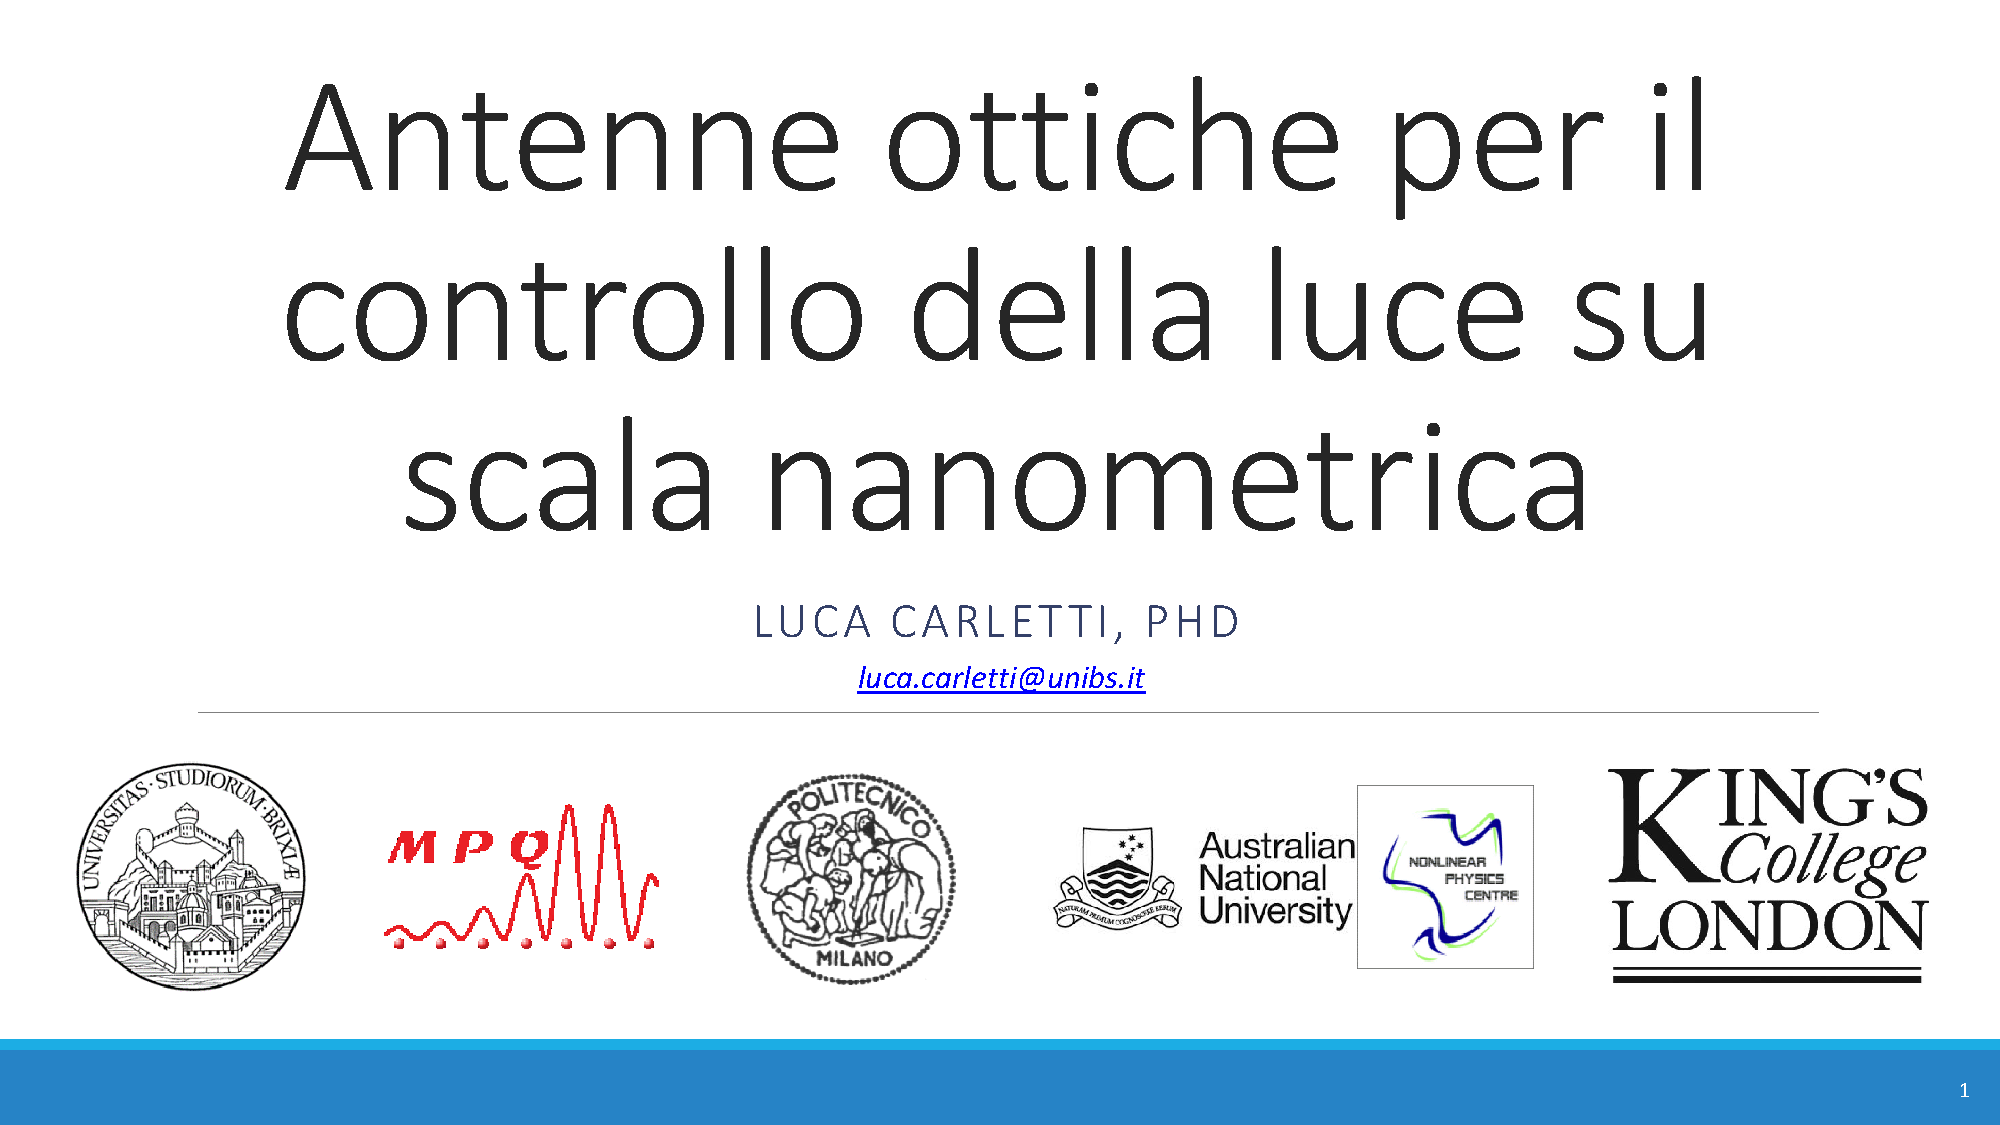
\includegraphics[page=1,scale=0.45]{slides/LucaCarletti_Nanoantenne.pdf}}

% 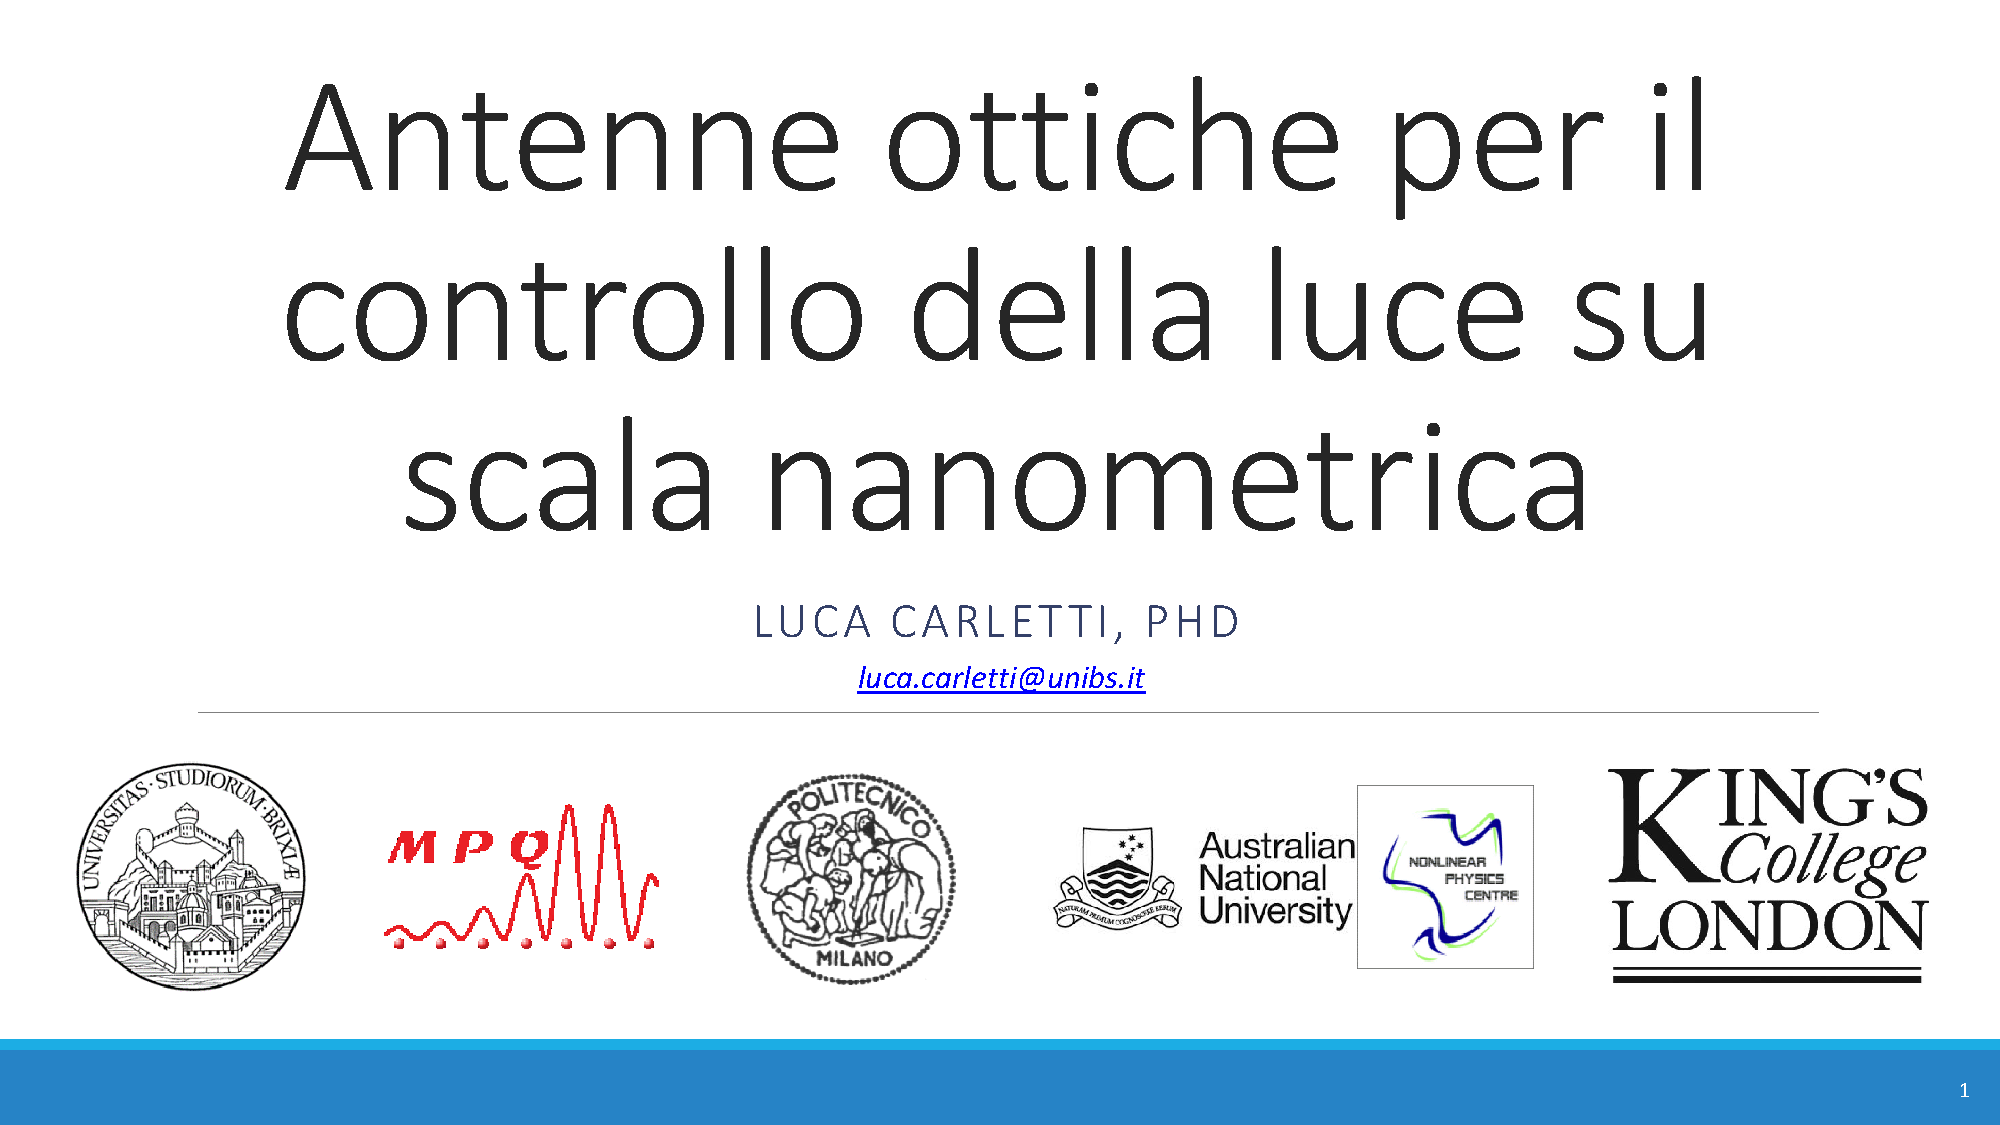
\includepdf[pages={1},nup=1x1,noautoscale=true,scale=0.6]{slides/LucaCarletti_Nanoantenne.pdf}
\includepdf[pages={2-},nup=1x2,noautoscale=true,scale=0.55]{slides/LucaCarletti_Nanoantenne.pdf}

\end{document}

%%% Local Variables:
%%% mode: latex
%%% TeX-master: t
%%% End:
